%%%%%%%%%%%%%%%%%%%%%%%%%%%%%%%%%%%%%%%%%%%%%%%%%%%%%%%%%%%%
%%% ELIFE ARTICLE TEMPLATE
%%%%%%%%%%%%%%%%%%%%%%%%%%%%%%%%%%%%%%%%%%%%%%%%%%%%%%%%%%%%
%%% PREAMBLE 
\documentclass[9pt,lineno,final]{elife}
% Use the onehalfspacing option for 1.5 line spacing
% Use the doublespacing option for 2.0 line spacing
% Please note that these options may affect formatting.
% Additionally, the use of the \newcommand function should be limited.


\usepackage{lipsum} % Required to insert dummy text
\usepackage[version=4]{mhchem}
\usepackage{siunitx}
\usepackage[color=green!30, textsize=small]{todonotes}
\usepackage{float}
\usepackage{graphicx}
\usepackage{subfig}
\usepackage{grffile}

\usepackage{array}
\usepackage[section]{placeins}
\usepackage{algorithm2e}
\usepackage{cleveref} % use \cref or \Cref to refer to labeled elements for automatically referring to the right type of entity, with the right capital letter and/or abbreviation rules
\usepackage[subpreambles=true]{standalone}
% \usepackage{endfloat}
\DeclareSIUnit\Molar{M}

\newcommand{\pH}{\mathrm{pH}}
\newcommand{\pKa}{\mathrm{pKa}}

% var for storing a box size
\newsavebox{\measurebox}

% Hidden table column
\newcolumntype{H}{>{\setbox0=\hbox\bgroup}c<{\egroup}@{}}
%%%%%%%%%%%%%%%%%%%%%%%%%%%%%%%%%%%%%%%%%%%%%%%%%%%%%%%%%%%%
%%% ARTICLE SETUP
%%%%%%%%%%%%%%%%%%%%%%%%%%%%%%%%%%%%%%%%%%%%%%%%%%%%%%%%%%%%
\title{Predicting pKa values and titration curves for the SAMPL6 pKa challenge using Epik and Jaguar}

\author[1,2]{Ari\"{e}n S. Rustenburg}
\author[1]{Mehtap Isik}
\author[1,2]{Patrick B. Grinaway}
\author[1,3]{Andrea Rizzi}
%\author[]{Art Bochevarov}
%\author[]{John Shelley}
\author[4]{Marilyn R Gunner}
\author[1*]{John D. Chodera}

\affil[1]{Computational and Systems Biology Program, Sloan Kettering Institute, Memorial Sloan Kettering Cancer Center, New York, NY 10065}
\affil[2]{Graduate Program in Physiology, Biophysics, and Systems Biology, Weill Cornell Medical College, New York, NY 10065}
\affil[3]{Tri-Institutional Training Program in Computational Biology and Medicine, New York, NY 10065}
\affil[4]{Department of Physics, City College of New York, New York, NY 10031}
\corr{john.chodera@choderalab.org}{JDC}

%\presentadd[\authfn{3}]{Schr\"{o}dinger, New York, NY 10036}

%\contrib[\authfn{1}]{These authors contributed equally to this work}
%\contrib[\authfn{2}]{These authors also contributed equally to this work}

%%%%%%%%%%%%%%%%%%%%%%%%%%%%%%%%%%%%%%%%%%%%%%%%%%%%%%%%%%%%
%%% ARTICLE START
%%%%%%%%%%%%%%%%%%%%%%%%%%%%%%%%%%%%%%%%%%%%%%%%%%%%%%%%%%%%

\begin{document}

\maketitle
%\tableofcontents
%\listoffigures
%\listoftables
\begin{abstract}
	The goal of the SAMPL6 pKa Challenge was to evaluate the performance of small molecule pKa prediction methods from challenge participants in a blinded fashion on a set of small, drug-like molecules resembling kinase inhibitor fragments.
	%
	To provide a useful point of comparison for blind participant predictions that may use experimental methods still under development, we performed reference benchmark calculations using a popular empirical model (Epik) and quantum chemical approach (Jaguar) from Schrödinger.
	%
	Epik predicts microstate populations and pKa values using a Hammett-Taft type model, while Jaguar is a fast DFT quantum chemical method.
	%
	In this work, we discuss how these reference calculations were performed, provide a broad assessment of the performance of the method, and highlight challenges and considerations in predicting pKa values to benchmark against experiment macroscopic pKa measurements.
\end{abstract}


\section{Introduction}

\todo[inline, color=red!90]{Still need to regenerate figures and tables containing last macroscopic data, after working out some bugs and experimenting with different ways of converting. Will update captions afterwards}

Titratable sites are ubiquitous in druglike small molecules.
%
Large-scale computational surveys suggest that 60\% of all protein-ligand complexes undergo a change in ionization state upon binding~\cite{Aguilar2010}, either due to protonation state changes of the small molecule or the protein (where roughly a third of all protein residues are ionizable~\cite{Jordan2005}).
%
More generally, protonation state effects---in which the dominant protonation, charge, or tautomer state shifts upon binding, or a mixture of protonation states are significantly populated in complex or solution---has the potential to cause large modeling errors if these effects are neglected. \cite{Martin2009, Greenwood2010,Bax2017}
%
In the SAMPL5 distribution coefficient (logD) challenge, for example, protonation state effects were determined to be a major contributor to loss in accuracy for the otherwise mundane task of predicting a transfer free energy between aqueous and cyclohexane phases~\cite{Pickard2016}.

To isolate the question of how well pKa effects could be modeled---and therefore how accurately the community could address these effects---the SAMPL6 challenge featured a blind pKa prediction component, as an intermediate step to logD predictions in which we provide participants with pKa values and later have them predict both pKa and logD~\cite{sampl6-pKa-measurements}.
The SAMPL6 pKa challenge consisted of predicting macroscopic pKa values measured by UV-metric titration for a set of small moelcules that resembled kinase inhibitors and their fragments~\cite{sampl6-pKa-measurements}.
As participants in the SAMPL6 pKa challenge were expected to utilize a wide variety of methods still under development, we endeavored to provide a useful baseline reference set of predictions using well-established, widely-deployed, commercially available methods.
We selected both an empirical method (Epik~\cite{Shelley2007Epik}) and quantum chemical method (Jaguar~\cite{Bochevarov2013}) from the Schr\"{o}dinger Suite of computational chemistry software, version 2017-4.

Reference calculations---which were not fully blinded---were performed in a manner that attempted to mimic standard use, using recommended settings for each program, without significantly modifying the input parameters.
As the computation of UV-metric macroscopic pKa values from the microscopic pKa values predicted by the tools is not necessarily completely straightforward, we considered several alternative possibilities, which we discuss in more detail.
We provide an analysis and broad assessment of the performance of the two methods, and highlight challenges and considerations in predicting pKa values to benchmark against experiment.
All analysis tools used to perform this study are available via GitHub at
\url{https://github.com/choderalab/SAMPL6-Reference-pKa-Calculations}

\section{Technology}


\subsection{Epik}

Epik\cite{Shelley2007Epik} is a program for predicting the pKa values of ionizable sites in druglike molecules and for generating their probable protonation states. Epik implements the empirical Hammett-Taft (HT) approach \cite{Perrin1981HammettTaft}  to rapidly estimate the pKa values of Brønsted acidic or basic functional groups identified by SMARTS \cite{SMARTSDaylight} patterns. The popular HT method describes a linear free energy relationship,

\begin{equation}
 pK_{a_i} = pK_{a_i}^0 - \rho_i  \sum_j \sigma_i \quad ,
\end{equation}

between an ionizable functional group reference $pK_{a_i}^0$ value, how sensitive ($\rho_i$) the group is to substituent perturbation, and how strongly ($\sigma_j$) each substituent, j, perturbs the pKa value. Epik’s internal $pK_{a_i}^0$, $\rho$ , and $\sigma$  parameters are fit to experimental data, or, rarely, to high-quality Jaguar calculations when experiments are unavailable.

Given a target pH and pH tolerance, the molecule can be appropriately protonated or deprotonated based on the estimated pKa values of its ionizable groups to generate the probable protonation states. The estimated pKa value of each functional group in a molecule is often exclusive to a specific tautomeric, protonation, and ionization state. Each (de)protonation can give rise to a set of tautomers and subsequent ionization states, all of which are iteratively generated and estimated until either exhausted or the predicted pKa values of the ionizable sites fall outside the tolerance range. Finally, the microscopic populations and corresponding free energy penalties are calculated and reported. Please note that Epik reports only microscopic pKa values, not macroscopic, or apparent pKa values.

\subsection{Jaguar}

Jaguar uses an \textit{ab initio} DFT method for calculating pKa values from 3 dimensional structures. It requires specification of pairs of protonated and deprotonated states and performs a free energy calculation between them. Specifically, it attempts to estimate the pKa using the free energy of deprotonation in solvent

\begin{align}
 pK_a = \frac{\Delta G_\textrm{(aq)}}{RT \ln 10}  
\end{align}

To estimate $ \Delta G_\textrm{(aq)}$, Jaguar depends on the following thermodynamic cycle:
%
\begin{figure}[H]
\centering
 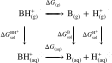
\includegraphics{jaguar-reaction}
\end{figure}
%
. From this thermydynamic cycle, the equation that produces the pKa can be derived:
%
\begin{equation}
 \Delta G_\textrm{(aq)} = \Delta G_\textrm{(g)} - \Delta G^\textrm{\ce{BH+}}_\textrm{sol} + \Delta G^\textrm{\ce{B}}_\textrm{sol}  +  \Delta G^\textrm{\ce{H+}}_\textrm{sol} \quad .
\end{equation}

It follows that when the 4 terms on the right are known, the pKa value can be estimated.
%
$\Delta G^\textrm{\ce{H+}}_\textrm{sol}$ has previously been established to be -259.5 kcal per mol\cite{Lim1991protonsolvation}.
%
Gas phase term $\Delta G_\textrm{(g)}$ is calculated using
%
\begin{equation}
 \Delta G_\textrm{(g)} = E_\textrm{\ce{B_{(g)}}} - E_\textrm{\ce{BH+ _{(g)}}} + \frac{5RT}{2 } - T \Delta S \quad .
\end{equation}

The values for $\frac{5RT}{2}$ and  - $T \Delta S$ are approximated to be 1.48 kcal per mol and 7.76 kcal per mol, assuming room temperature and 1 atm pressure.~\cite{Bochevarov2016multiconformation}

The energy terms require first a geometry optimization, which is performed using B3LYP/6-31G*. 
%
Afterwards, B3LYP/cc-pVTZ+ is used for atoms involved in the deprotonation reaction, and the remainder are treated using the cc-pVTZ basis set.
%
\todo[inline]{ASR: Describe solvation calculation and need for empirical correction}

\todo[inline]{ASR: Describe how multiple conformations are incorporated}
\todo[inline]{ASR:Explain the individual terms in the equations above, citations for method}

\section{Analysis}

\subsection{Predicting macroscopic pKa values}


Epik and Jaguar predict microscopic pKa values or microstate energies, which must be translated into macroscopic pKa values for comparison to experiment.
Several choices are possible for comparing these microscopic properties into macroscopic pKa values.
%

\begin{figure}[H]
	\centering
	
	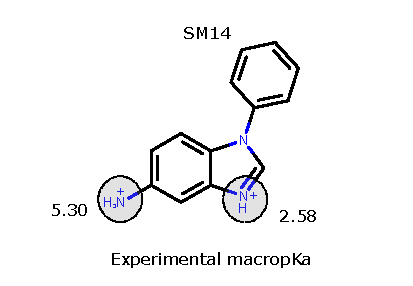
\includegraphics[width=0.47\textwidth]{Images/Molecules/SM14-pka.pdf} \hfill
	
	\begin{gather*}
\begin{bmatrix} \pi_{1} \\ \pi_{2} \\ \pi_{n} \\ \vdots \\ \vdots \\ \pi_{m} \\ \pi_{m+1}\\ \end{bmatrix}
=
\begin{bmatrix}
 1       & 1       & 1       & 1       & \cdots    & 1& 1  & 1 \\
 K_{a,1} & -H      & 0       & 0       & \cdots    & 0&0  & 0 \\
 0       & K_{a,2} & -H      & 0       & \cdots    & 0&0  & 0 \\
 0       & 0       & K_{a,n} & -H      & \cdots    & 0&0  & 0 \\  
 \vdots  & \vdots  & \vdots  & \vdots  & \ddots    & \vdots & \vdots  & \vdots \\
 0       & 0       & 0       & 0       & \cdots    & K_{a,m} & -H & 0 \\  
 0       & 0       & 0       & 0       & \cdots    &         0    & K_{a,m+1}   & -H \\
\end{bmatrix}^{-1}
\begin{bmatrix} \sum_{i=1}^{m+1} \pi_i \\ 0 \\ 0 \\ \vdots \\ \vdots \\ 0 \\ 0\\ \end{bmatrix}\\
\end{gather*}
    \hfill
	\includegraphics[width=0.47\textwidth]{fig2_population_sm14.pdf}
	\includegraphics[width=0.47\textwidth]{fig2_charge_sm14.pdf} \\
 	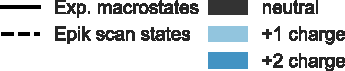
\includegraphics[width=0.4\textwidth]{fig2_legend}
	\todo[inline]{Fix this figure, make it with macroscopic estimates}
		\caption{{\bf Macroscopic pKa values can be directly compared to experimental values. Additionally, a populations and the charge titration curve can be compared.} Molecule SM07 pKa values were measured using UV (citation) for the purpose of the SAMPL6 challenge, and based on a subsequent NMR experiment the identity of the microstates were identified. In this example, we show the results produced by Epik scan to for illustration.
	\label{fig:scan-prediction}}
	
\end{figure}


It is possible to translate the micropKas into macropKas
\cite{Bochevarov2016multiconformation, Philipp2018macropka}

\begin{align}
 K_a^\text{macro} = \sum_{j=1}^{N_\text{deprot}} \frac{1}{\sum_{i=1}^{N_\text{prot}}\frac{1}{ K_{ij^\text{micro}}}} \label{eq:macropka}
 \end{align}

\todo[inline]{Update tables and also add the macroestimates obtained using this equation}
 

 
\subsection{Population curves from pKa}
One way to estimate the performance of a pKa prediction method is to look at the population curves.
%
To generate a population ($\pi_i$) for a state $i$ from a pKa value one first needs to convert the pKa values (microscopic or macroscopic), one can make use of the sequential equilibrium constants 
%
\begin{align}
 \frac{K_{a,i}}{10^{-pH}} = \frac{\pi_{i+1}}{\pi_{i}}
\end{align}

to construct a system of equations. The macroscopic equations can be represented as a matrix equation \textcolor{green}{add citation}
%
\begin{gather}
\begin{bmatrix} \pi_{1} \\ \pi_{2} \\ \pi_{n} \\ \vdots \\ \vdots \\ \pi_{m} \\ \pi_{m+1}\\ \end{bmatrix}
=
\begin{bmatrix}
 1       & 1       & 1       & 1       & \cdots    & 1& 1  & 1 \\
 K_{a,1} & -H      & 0       & 0       & \cdots    & 0&0  & 0 \\
 0       & K_{a,2} & -H      & 0       & \cdots    & 0&0  & 0 \\
 0       & 0       & K_{a,n} & -H      & \cdots    & 0&0  & 0 \\  
 \vdots  & \vdots  & \vdots  & \vdots  & \ddots    & \vdots & \vdots  & \vdots \\
 0       & 0       & 0       & 0       & \cdots    & K_{a,m} & -H & 0 \\  
 0       & 0       & 0       & 0       & \cdots    &         0    & K_{a,m+1}   & -H \\
\end{bmatrix}^{-1}
\begin{bmatrix} \sum_{i=1}^{m+1} \pi_i \\ 0 \\ 0 \\ \vdots \\ \vdots \\ 0 \\ 0\\ \end{bmatrix}
\end{gather}
%
Note that in our case, $\sum\limits_{i=1}^{m+1} \pi_i \equiv 1$, but if one is dealing with actual concentrations, one can use the total concentration of the compound to receive concentrations instead of populations.

For microscopic states, one can constructing a similar matrix, but very often there is no solution to the equation as one ends up with a singular matrix. 
%
For directly predicting microscopic populations, instead we derive them based on free energies. 
%
The free energy of a single state is defined 
\begin{eqnarray}
	g_i(\pH) &=& \beta \left( n_i*\pH - \sum_j \pKa_j \right) \label{eq:pkatodg}
\end{eqnarray}
%
, where $\beta$ is the inverse temperature, and the index $j$ indicates all protonation states in between the most deprotonated state and state $i$. 
%
For macroscopic pKa values, this is straightforward.
%
In the case of microscopic pKa values, when more than one combinations of pKa values exist, the pKa path with the smallest standard error is chosen.
%
Since the free energy is a state function, it should not depend on the path of reactions taken.
%
In practice, since pKa values are produced individually, one might get a slightly different answer depending on the path chosen.
%

It is common to select one state as a reference state, and set its free energy to zero, whilst subtracting it's free energy from the other states.
%
We choose to set the free energy reference to be a neutral state, since this means the slope of the free energy with respect to pH will be equal to the charge of the species, which is illustrative.

After obtaining normalized free energies, the populations $\pi_i$ of each state are derived in a familiar way, by Boltzmann weights

\begin{eqnarray}
	\pi_i(\pH) &=& \frac{e^{-g_i(\pH)}}{\sum_i e^{-g_i(\pH)} } \label{eq:dgtopi}
\end{eqnarray}

This provides us with a pH-dependent population for each microstate.


\subsection{Virtual electrochemical titration}

From the previous section, we know the populations of individual microstates, $\pi_i$. 
%
We can combine this with the charge of the individual microstates to generate a potentiometric titration curve.
%


\begin{eqnarray}
	\langle q_\text{total} \rangle (\pH) = \sum_i q_i \times \pi_i(\pH) 
\end{eqnarray}

An alternative way to express this is using matrix multiplication.
%
We define $\mathbf{q}$ as a column vector of $N$ charges, $q_i$ for each state $i$.
%
Then, if we take $\boldsymbol{\Pi}$ to be a matrix of $M$ pH values by $N$ states,
%
We can simply take the matrix product to achieve the same.
\begin{align}
    \langle q_\text{total} \rangle (\pH) = \mathbf{q} \boldsymbol{\Pi} 
\end{align}




\begin{itemize}
	\item Sequential titration avoids the need to compute the energies of \emph{all} protonation states
	\item Epik can automatically perform a sequential scan (which can also be used in Jaguar with some automation)
	\item For this experiment, we started from the predicted highest-occupancy microstate at pH 7 and went in both directions, returning pKa values between 2-12
	\item Average charge vs pH to match electrochemical titrations, look at the mean signed deviation (MSD) or area between curves to see whether the charge curve behavior matches
\end{itemize}

\subsection{Directly from microstate predictions}

Methods like Epik and Jaguar provide microstate pKa predictions.
%
This means that rather than macroscopic pKas observed in the average charge state (potentiometric titration) or number of titration events (UV titration curve), it produces a microequilibrium constant between a single pair of configurations (protonation states or tautomers) is predicted. 
%
One way to compare experiment and prediction is by directly comparing 
pKa values.
%
However, there are likely many microstates, and only a few macrostates.
%
Therefore, we also look at the predicted titration curve, which can incorporate information from every microstate into a macrostate.


\begin{figure}
\centering
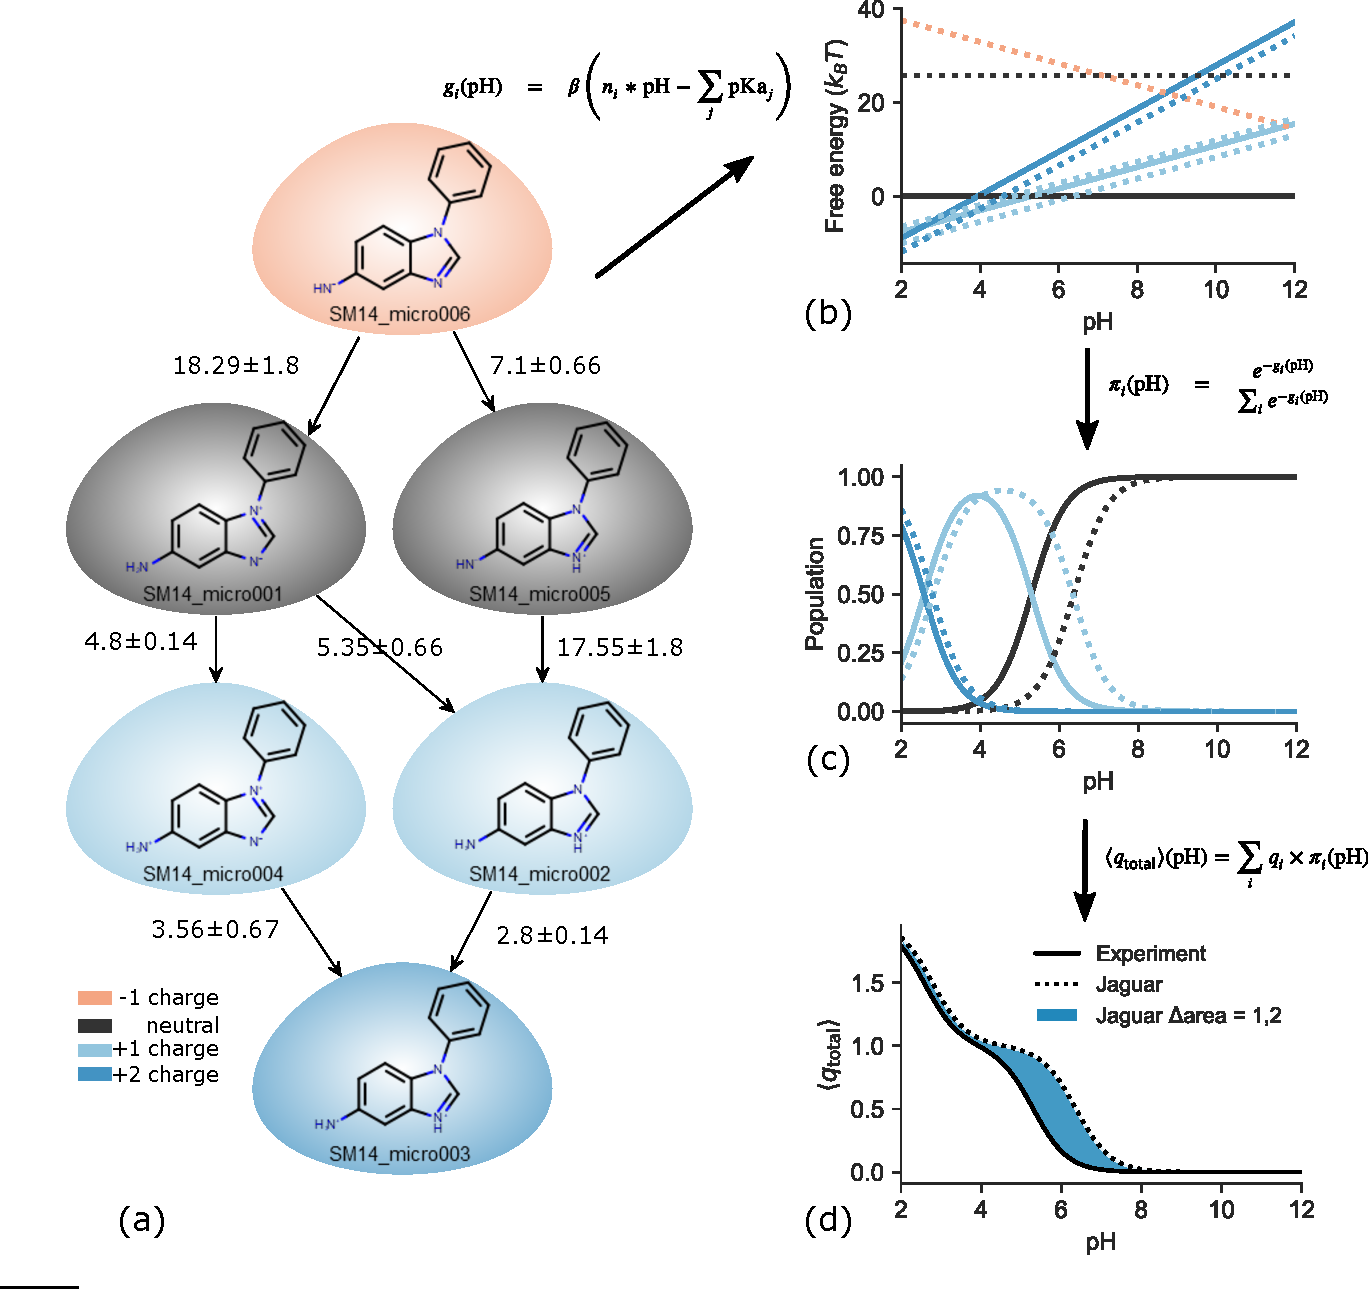
\includegraphics[width=\textwidth]{micropka-workflow.pdf}
\caption{{\bf Workflow for directly converting microscopic pKa values into a macroscopic titration curve.} Microscopic pKa predictions {\bf(a)} can be translated into free energies {\bf(b)} using Equation \ref{eq:pkatodg} and then into populations {\bf(c)} using Equation \ref{eq:dgtopi}. When one combines this with the charges for each microstate, one can generate the mean charge titration curve {\bf(d)}. The example shown is the Jaguar prediction for SM14.
	\label{fig:sm14-prediction}}
\end{figure}


\subsection{pKa matching algorithms}
The experiments do not provide any microscopic information on what atom, or microstate a pKa belongs to.
%
Therefore, it is necessary to perform a matching of pKa values between experiment and predicted pKa values.
%
There are several ways one could go about this, each strategy can prioritize a different aspect to match.
%
Although the experimental values are macroscopic, comparing to microscopic pKas might give us insight into which microstates produce the macroscopic signature observed in the experiment.
%
We can also compare macroscopic pKas, either produced by Epik scan, or using \cref{eq:macropka}, directly to experimental values.
%

We consider three algorithms that emphasize different :

\begin{itemize}
 \item closest match
 \item Hungarian match (linear sum assignment)
 \item sequential match
\end{itemize}

which are described in the following three sections

\subsection{Closest pKa matching}

We systematically look for all possible pairings of pKa values, and assign them sequentially. 

\begin{figure}[H]

\begin{algorithm}[H]
	\SetAlgoLined
	\caption{This algorithm matches experiment with prediction based on how close each value is, one pKa value at a time. Unless the matrix $C$ is square, some values will be unmatched. Those leftover pKa values are returned at the end. It uses a cost function, such as root mean square deviation, to assess how close two values are.}
	\label{alg:closest}
	\KwResult{Mapping of each experimental pKa $i$ to predicted pKa $j$}
	 
	$C$ is constructed, where every row  $i$ is an experiment, and every column $j$ a prediction\;
	$C_{ij}$ = cost($\pKa_{\text{exp},i}$, $\pKa_{\text{pred},j}$)\;
	\While{$C$.size > 0}{
		$k, l$ = arg min($C_{ij}$)\;
		assign experimental value $k$ to prediction $l$\;
		remove row $k$, column $l$ from $C$;\
	}
	remaining values are unmatched\;

\end{algorithm}
\end{figure}


\subsection{Hungarian pKa matching}
This algorithm, also known as linear sum assignment.
%
It finds the combination of pKa that minimizes the overall cost by picking rows and columns in a matrix, also considering the cost of not mapping certain pKa values in the case of different numbers of predictions and experimental values.
%
It is subtly different from the closest algorighm, as it looks for an overall minimized cost, rather than judging individual pKa costs, one at a time. 
%
In practice, the results may be similar to the closest algorithm.

\subsection{Sequential pKa matching}

For macroscopic only, because it doesn't make sense to sequentially align microscopic pKa values to a set of macroscopic pKa values. 
%
This algorithm is used because it should follow physically that protonation state constants would be sequentially adding charge/protons.
%
When comparing macroscopic pKa values, we therefore would wish to constrain the matching of pKa values to be sequential. For this we use \cref{alg:sequential}.

\begin{figure}[H]
	\begin{algorithm}[H]
		\SetAlgoLined
		\caption{Sequential pKa mapping. It uses a cost function to measure cost, and it rolls (shifts by one, and reintroduces last element as first). Any unmatched pKa values are represented by matching with a placeholder value. To calculate the cost, the placeholder is replaced by either 0, or 14, depending on whether the unmatched value is above or below 7.0.}
		\label{alg:sequential}
		\KwResult{Mapping of each experimental pKa $i$ to predicted pKa $j$}
		 
		$I$ = sorted experimental pKa values \;
		$J$ = sorted predicted pKa values \;
		length = max($I$.size, $J$.size)\;
		Append placeholders such that $I$.size = length \;
		Append placeholders such that $J$.size = length \;
		min = $\infty$\;
		solution = J rolled 0 times\;
		\For{n in 0..length}{
			$S$ = J rolled n times \;
			total = 0.0\;
			\For{m in 0..length}{				
				total = total + cost($I_m$, $J_m$)\;
			}
			\If(solution is better){total < min}{
				min = total\;
				solution = S \;
			}		}
	\end{algorithm}
\end{figure}

\section{Results}

\subsection{Overall performance}

- Based on what we've seen in early overview assessments, Epik scan performed in the top-5 of methods out there, and Jaguar seems to perform better than Epik in our work here. Epik microscopic pKa values are also performing better than just using scan mode.

- Jaguar performs best of all methods we considered here. It has the strongest pKa correlations, and the titration curves are most likely to be correct.
- It did not perform well for a few outliers (SM18), perhaps due to the many different microstates, the accumulation of errors is large.


- Epik performs similarly to Jaguar, but doesn't return as many protonation states/pKas. This might be a blessing and a curse. Sometimes, Epik might miss relevant microstates, while sometimes,
it avoids states it has not been parametrized for. That said,
when Epik is told to return low-probability structures, it can return
problematic configurations of the molecule (see also Discussion).

- Epik scan performs surprisingly well. In the initial overview, it was shown to be in the top 5 of predictors of the entire SAMPL6 challenge.


\begin{table}[H]
\centering
	\caption{{\bf Overall performance of each method} using either the closest pKa matching, Hungarian pKa matching, or sequentially aligned pKa values, and the area between the experimental and predicted macroscopic charge titration curve}
	\label{tab:overview-performance}
\todo[inline]{Add area back into this table}
\begin{tabular}{lll}
\toprule
       Method &             Metric &                 Value \\
\midrule
  Epik macro &               RMSE &        1.0 [0.9, 1.1] \\
  Epik macro &    Mean abs. error &        0.8 [0.7, 0.9] \\
  Epik macro &     pearson $\rho$ &     0.93 [0.91, 0.96] \\
  Epik macro &  Median abs. error &        0.7 [0.5, 0.9] \\
  Epik micro &               RMSE &        0.7 [0.6, 0.9] \\
  Epik micro &    Mean abs. error &        0.5 [0.4, 0.6] \\
  Epik micro &     pearson $\rho$ &     0.96 [0.92, 0.98] \\
  Epik micro &  Median abs. error &        0.3 [0.2, 0.4] \\
   Epik scan &               RMSE &        0.9 [0.8, 1.1] \\
   Epik scan &    Mean abs. error &        0.8 [0.6, 0.9] \\
   Epik scan &     pearson $\rho$ &     0.94 [0.89, 0.97] \\
   Epik scan &  Median abs. error &        0.7 [0.5, 0.8] \\
Jaguar macro &               RMSE &        1.1 [0.8, 1.3] \\
Jaguar macro &    Mean abs. error &        0.8 [0.6, 0.9] \\
Jaguar macro &     pearson $\rho$ &     0.94 [0.91, 0.97] \\
Jaguar macro &  Median abs. error &        0.7 [0.6, 0.8] \\
Jaguar micro &               RMSE &     0.47 [0.31, 0.54] \\
Jaguar micro &    Mean abs. error &        0.3 [0.2, 0.4] \\
Jaguar micro &     pearson $\rho$ &  0.986 [0.971, 0.994] \\
Jaguar micro &  Median abs. error &     0.21 [0.15, 0.25] \\
\bottomrule
\end{tabular}
\end{table}


Overall performance of Epik and Jaguar based on various metrics (figures/tables)
\subsubsection {Matching of experimental and calculated pKa values}




%

\begin{table}[H]
\centering
 \caption{{\bf Mean charge titration curve comparison with respect to experiment ($\Delta$ area) with confidence intervals.} Confidence intervals were obtained by gaussian bootstrapping over pKa values from the standard errors reported by the software.}\label{tab:titrationcurves}
\begin{tabular}{llllll}
\toprule
{} &       Epik-micro &         Epik-macro &          Epik-scan &    Jaguar-micro &       Jaguar-macro \\
\midrule
SM01     &   0.5 [0.2, 4.8] &     0.4 [0.1, 3.0] &     0.5 [0.1, 4.0] &  1.1 [0.1, 4.2] &     0.2 [0.0, 1.7] \\
SM02     &   2.1 [0.2, 3.2] &     0.9 [0.1, 4.0] &     1.9 [0.7, 4.0] &  1.6 [0.3, 4.9] &     1.3 [0.2, 4.5] \\
SM03     &   1.5 [0.6, 5.1] &  0.11 [0.12, 4.52] &  0.10 [0.07, 4.67] &  0.5 [0.7, 4.9] &     0.3 [0.1, 3.8] \\
SM04     &   2.6 [0.1, 4.0] &     0.4 [0.1, 3.5] &     2.2 [0.3, 4.9] &  1.1 [0.1, 4.0] &     0.8 [0.1, 2.7] \\
SM05     &   2.2 [0.4, 4.8] &     1.1 [0.2, 4.6] &     1.1 [0.3, 4.7] &  0.2 [0.1, 3.9] &     0.4 [0.0, 1.3] \\
SM06     &  2.2 [0.6, 10.0] &     2.6 [0.6, 6.9] &     2.6 [0.6, 7.0] &  1.3 [0.5, 4.8] &     2.1 [1.1, 3.0] \\
SM07     &   2.6 [0.1, 4.1] &     0.5 [0.1, 3.5] &     2.2 [0.8, 4.8] &  0.8 [0.1, 4.1] &     0.7 [0.0, 2.6] \\
SM08     &   1.2 [0.4, 6.7] &     0.6 [0.3, 5.4] &     0.6 [0.3, 6.5] &  7.1 [3.0, 9.4] &     4.5 [2.7, 6.1] \\
SM09     &   2.5 [0.2, 3.5] &     1.2 [0.1, 3.2] &     2.3 [0.6, 3.7] &  1.0 [0.2, 4.4] &     0.7 [0.1, 3.6] \\
SM10     &   0.6 [0.2, 5.4] &     0.4 [0.1, 3.9] &     0.6 [0.2, 5.7] &  0.3 [0.1, 5.2] &     0.2 [0.0, 2.0] \\
SM11     &   1.9 [0.2, 3.8] &  0.05 [0.10, 3.55] &     0.1 [0.2, 4.8] &  3.9 [0.3, 7.1] &     1.6 [0.2, 4.7] \\
SM12     &   2.5 [0.2, 3.7] &     1.2 [0.1, 4.4] &     2.2 [0.8, 4.1] &  0.9 [0.2, 4.9] &     2.1 [0.6, 4.7] \\
SM13     &   2.6 [0.1, 3.9] &     1.4 [0.1, 3.8] &     2.8 [0.4, 5.0] &  0.5 [0.1, 4.0] &     0.3 [0.0, 2.7] \\
SM14     &   1.0 [0.6, 6.0] &     1.7 [0.7, 5.2] &     1.8 [0.5, 5.6] &  1.2 [0.1, 3.6] &     0.3 [0.2, 3.8] \\
SM15     &   1.1 [0.4, 4.4] &     1.3 [0.5, 4.6] &     1.3 [0.5, 4.3] &  0.3 [0.2, 2.6] &     0.3 [0.2, 2.5] \\
SM16     &   2.9 [0.6, 4.8] &     1.4 [0.6, 4.8] &     1.4 [0.5, 4.8] &  1.5 [0.4, 4.6] &     1.0 [0.3, 3.2] \\
SM17     &   1.7 [0.3, 3.2] &     1.7 [0.3, 3.2] &     1.7 [0.3, 3.1] &  0.1 [0.0, 1.4] &  0.08 [0.06, 3.81] \\
SM18     &   0.8 [1.0, 9.7] &     0.7 [0.6, 5.8] &     1.0 [0.9, 8.4] &  2.2 [1.4, 6.9] &     1.6 [0.7, 3.8] \\
SM19     &   0.7 [0.1, 5.3] &     0.4 [0.1, 4.1] &     0.7 [0.2, 5.9] &  1.8 [0.3, 6.8] &     0.9 [0.1, 3.7] \\
SM20     &   2.3 [0.1, 4.9] &     2.3 [0.1, 4.9] &     2.3 [0.1, 4.9] &  1.6 [0.1, 3.5] &     1.6 [0.1, 3.4] \\
SM21     &   2.2 [0.6, 6.6] &     0.3 [0.1, 4.6] &     0.5 [0.3, 6.5] &  1.6 [0.6, 7.1] &     2.5 [0.6, 5.0] \\
SM22     &   1.6 [0.4, 4.6] &     1.6 [0.5, 4.4] &     1.6 [0.4, 3.9] &  0.2 [0.1, 2.9] &     0.6 [0.3, 4.0] \\
SM23     &   0.4 [0.1, 3.4] &     0.6 [0.1, 2.4] &     3.1 [1.6, 5.0] &  2.1 [1.2, 5.7] &     3.6 [2.9, 4.4] \\
SM24     &   3.6 [0.2, 5.2] &     3.5 [1.5, 5.0] &     5.6 [3.1, 9.3] &  2.3 [0.2, 5.3] &     0.8 [0.1, 4.3] \\
\bottomrule
\end{tabular}
 
\end{table}



\begin{figure}[hbtp]
	\centering
	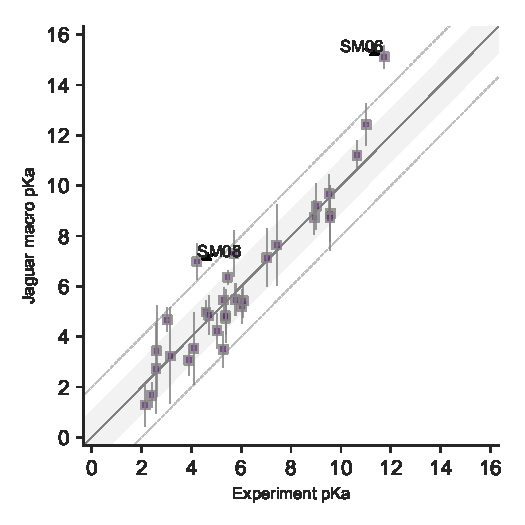
\includegraphics[]{Reports/Experiment-Jaguar-macro-align-correlation.pdf}	
	\caption{{\bf Jaguar macroscopic pKa values compared to macroscopic experimental pKa values, sequentially matching pKa values}  Gray bands denote one pKa unit difference, while the dashed lines indicate two pKa units. Outliers with more than 2 pKa units deviation are labeled.}
\end{figure}

\begin{figure}[hbtp]
	\centering
	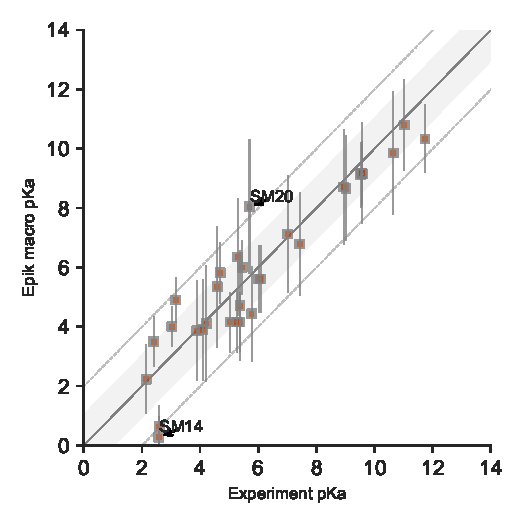
\includegraphics[]{Reports/Experiment-Epik-macro-align-correlation.pdf}	
	\caption{{\bf Epik macroscopic pKa values compared to macroscopic experimental pKa values, sequentially matching pKa values}  Gray bands denote one pKa unit difference, while the dashed lines indicate two pKa units. Outliers with more than 2 pKa units deviation are labeled.}
\end{figure}

\begin{figure}[hbtp]
	\centering
	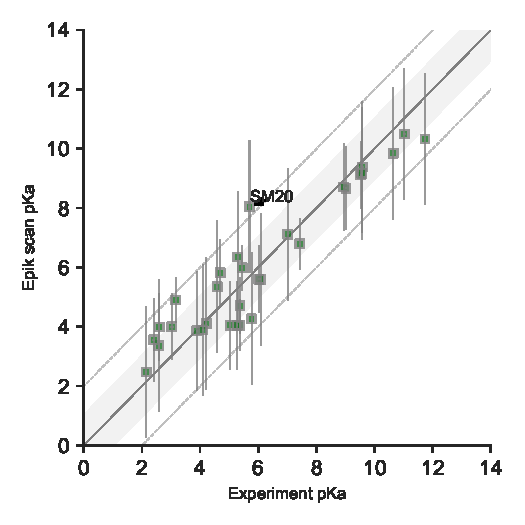
\includegraphics[]{Reports/Experiment-Epik-scan-align-correlation.pdf}	
	\caption{{\bf Epik scan pKa values compared to macroscopic experimental pKa values, sequentially matching pKa values}  Gray bands denote one pKa unit difference, while the dashed lines indicate two pKa units. Outliers with more than 2 pKa units deviation are labeled.}
\end{figure}


\begin{figure}
 \centering
 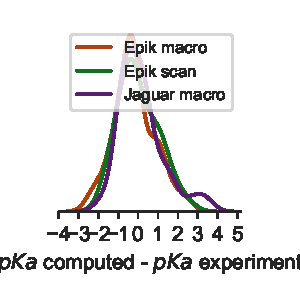
\includegraphics{Reports/overview-align-distribution.pdf}
 \caption{{\bf Distribution of the pKa errors for macroscopic estimates.} The difference (predicted - measured) are plotted as a gaussian kernel density estimate.}
\end{figure}


\begin{figure}
 \centering
 \includegraphics{Reports/Experiment-Jaguar-Macro-align-distribution.pdf}
 \caption{{\bf Distribution of the Jaguar pKa errors for macroscopic estimates.} The difference (predicted - measured) are plotted as a gaussian kernel density estimate with individual values as marks at the bottom. The median error is denoted by a vertical line.}
\end{figure}

\begin{figure}
 \centering
 \includegraphics{Reports/Experiment-Epik-Macro-align-distribution.pdf}
 \caption{{\bf Distribution of the Epik pKa errors for macroscopic estimates.} The difference (predicted - measured) are plotted as a gaussian kernel density estimate with individual values as marks at the bottom. The median error is denoted by a vertical line.}
\end{figure}

\begin{figure}
 \centering
 \includegraphics{Reports/Experiment-Epik-Scan-align-distribution.pdf}
 \caption{{\bf Distribution of the Epik pKa errors for macroscopic estimates.} The difference (predicted - measured) are plotted as a gaussian kernel density estimate with individual values as marks at the bottom. The median error is denoted by a vertical line.}
\end{figure}


\sisetup{separate-uncertainty=true}
\begin{table}
\centering
\small
\caption{{\bf Macroscopic pKa values assigned by sequential pKa alignment.}}
\label{tab:molecule-macro}
\rowcolors{2}{gray!25}{white}
\begin{tabular}{cS[table-format=-1.2,table-figures-uncertainty=1]S[table-format=-1.1,table-figures-uncertainty=1]S[table-format=-1.1,table-figures-uncertainty=1]S[table-format=-1.1,table-figures-uncertainty=1]S[table-format=-1.1,table-figures-uncertainty=1]S[table-format=-1.1,table-figures-uncertainty=1]S[table-format=-1.1,table-figures-uncertainty=1]S[table-format=-1.1,table-figures-uncertainty=1]S[table-format=-1.1,table-figures-uncertainty=1]S[table-format=-1.1,table-figures-uncertainty=1]S[table-format=-1.1,table-figures-uncertainty=1]S[table-format=-1.1,table-figures-uncertainty=1]S[table-format=-1.1,table-figures-uncertainty=1]}\toprule
{Molecule} &    {Experiment} & {Epik macro} & {Epik macro Delta} &  {Epik scan} & {Epik scan Delta} & {Jaguar macro} & {Jaguar macro Delta} \\
\midrule
      SM01 &   9.53 \pm 0.01 &      9 \pm 1 &           -0 \pm 1 &      9 \pm 1 &          -0 \pm 1 &    9.7 \pm 0.8 &          0.1 \pm 0.8 \\
      SM02 &   5.03 \pm 0.01 &      4 \pm 1 &           -1 \pm 1 &      4 \pm 1 &          -1 \pm 1 &    4.2 \pm 0.7 &         -0.8 \pm 0.7 \\
      SM03 &   7.02 \pm 0.01 &      7 \pm 2 &            0 \pm 2 &      7 \pm 2 &           0 \pm 2 &        7 \pm 1 &              0 \pm 1 \\
      SM04 &   6.02 \pm 0.01 &      6 \pm 1 &           -0 \pm 1 &      6 \pm 1 &          -0 \pm 1 &    5.2 \pm 0.7 &         -0.8 \pm 0.7 \\
      SM05 &   4.59 \pm 0.01 &      5 \pm 2 &            1 \pm 2 &      5 \pm 2 &           1 \pm 2 &    5.0 \pm 0.5 &          0.4 \pm 0.5 \\
      SM06 &   3.03 \pm 0.04 &  4.0 \pm 0.7 &        1.0 \pm 0.7 &      4 \pm 1 &           1 \pm 1 &    4.7 \pm 0.5 &          1.7 \pm 0.5 \\
      SM06 &  11.74 \pm 0.01 &     10 \pm 1 &           -1 \pm 1 &     10 \pm 2 &          -1 \pm 2 &   15.1 \pm 0.5 &          3.4 \pm 0.5 \\
      SM07 &   6.08 \pm 0.01 &      6 \pm 1 &           -0 \pm 1 &      6 \pm 2 &          -0 \pm 2 &    5.4 \pm 0.7 &         -0.7 \pm 0.7 \\
      SM08 &   4.22 \pm 0.01 &      4 \pm 2 &           -0 \pm 2 &      4 \pm 2 &          -0 \pm 2 &    7.0 \pm 0.7 &          2.8 \pm 0.7 \\
      SM09 &   5.37 \pm 0.01 &      4 \pm 1 &           -1 \pm 1 &  4.0 \pm 0.9 &      -1.3 \pm 0.9 &    4.7 \pm 0.7 &         -0.6 \pm 0.7 \\
      SM10 &   9.02 \pm 0.01 &      9 \pm 2 &           -0 \pm 2 &      9 \pm 1 &          -0 \pm 1 &    9.2 \pm 0.9 &          0.2 \pm 0.9 \\
      SM11 &   3.89 \pm 0.01 &      4 \pm 2 &           -0 \pm 2 &      4 \pm 2 &          -0 \pm 2 &    3.1 \pm 0.6 &         -0.8 \pm 0.6 \\
      SM12 &   5.28 \pm 0.01 &      4 \pm 1 &           -1 \pm 1 &      4 \pm 1 &          -1 \pm 1 &    3.5 \pm 0.7 &         -1.8 \pm 0.7 \\
      SM13 &   5.77 \pm 0.01 &      4 \pm 2 &           -1 \pm 2 &      4 \pm 2 &          -2 \pm 2 &    5.5 \pm 0.6 &         -0.3 \pm 0.6 \\
      SM14 &   2.58 \pm 0.01 &  0.3 \pm 0.7 &       -2.3 \pm 0.7 &      3 \pm 2 &           1 \pm 2 &        3 \pm 2 &              0 \pm 2 \\
      SM14 &   5.30 \pm 0.01 &      6 \pm 2 &            1 \pm 2 &      6 \pm 2 &           1 \pm 2 &    5.5 \pm 0.5 &          0.2 \pm 0.5 \\
      SM15 &   4.70 \pm 0.01 &      6 \pm 1 &            1 \pm 1 &      6 \pm 1 &           1 \pm 1 &    4.8 \pm 0.8 &          0.1 \pm 0.8 \\
      SM15 &   8.94 \pm 0.01 &      9 \pm 2 &           -0 \pm 2 &      9 \pm 1 &          -0 \pm 1 &    8.7 \pm 0.7 &         -0.2 \pm 0.7 \\
      SM16 &   5.37 \pm 0.01 &      5 \pm 2 &           -1 \pm 2 &  4.7 \pm 0.9 &      -0.7 \pm 0.9 &        5 \pm 1 &             -1 \pm 1 \\
      SM16 &  10.65 \pm 0.01 &     10 \pm 2 &           -1 \pm 2 &     10 \pm 2 &          -1 \pm 2 &   11.2 \pm 0.6 &          0.6 \pm 0.6 \\
      SM17 &   3.16 \pm 0.01 &  4.9 \pm 0.7 &        1.7 \pm 0.7 &  4.9 \pm 0.7 &       1.7 \pm 0.7 &        3 \pm 2 &              0 \pm 2 \\
      SM18 &   2.15 \pm 0.02 &      2 \pm 1 &            0 \pm 1 &      2 \pm 2 &           0 \pm 2 &    1.3 \pm 0.9 &         -0.9 \pm 0.9 \\
      SM18 &   9.58 \pm 0.03 &      9 \pm 1 &           -0 \pm 1 &      9 \pm 2 &          -0 \pm 2 &        9 \pm 1 &             -1 \pm 1 \\
      SM18 &  11.02 \pm 0.04 &     11 \pm 2 &           -0 \pm 2 &     10 \pm 2 &          -1 \pm 2 &   12.4 \pm 0.8 &          1.4 \pm 0.8 \\
      SM19 &   9.56 \pm 0.02 &      9 \pm 2 &           -0 \pm 2 &      9 \pm 2 &          -0 \pm 2 &        9 \pm 1 &             -1 \pm 1 \\
      SM20 &   5.70 \pm 0.03 &      8 \pm 2 &            2 \pm 2 &      8 \pm 2 &           2 \pm 2 &    7.3 \pm 0.9 &          1.6 \pm 0.9 \\
      SM21 &   4.10 \pm 0.01 &      4 \pm 2 &           -0 \pm 2 &      4 \pm 2 &          -0 \pm 2 &        4 \pm 1 &             -1 \pm 1 \\
      SM22 &   2.40 \pm 0.02 &  3.5 \pm 0.8 &        1.1 \pm 0.8 &      4 \pm 1 &           1 \pm 1 &    1.7 \pm 0.5 &         -0.7 \pm 0.5 \\
      SM22 &   7.43 \pm 0.01 &      7 \pm 2 &           -1 \pm 2 &  6.8 \pm 0.9 &      -0.6 \pm 0.9 &        8 \pm 2 &              0 \pm 2 \\
      SM23 &   5.45 \pm 0.01 &  6.0 \pm 0.9 &        0.5 \pm 0.9 &  6.0 \pm 0.8 &       0.5 \pm 0.8 &    6.4 \pm 0.3 &          0.9 \pm 0.3 \\
      SM24 &   2.60 \pm 0.01 &  0.6 \pm 0.7 &       -2.0 \pm 0.7 &      4 \pm 1 &           1 \pm 1 &        3 \pm 2 &              1 \pm 2 \\
\bottomrule
\end{tabular}
\end{table}


    

\subsection{Macroscopic titration curves}
\begin{itemize}
	\item Compare macroscopic titration results, see if microcurves are much different.
	\item different types of mistakes
	\begin{enumerate}
	 \item wrong pKa value 
	 \item too many pKa values (wrong total charges)
	 \item compare number of apparent pKas vs macropKas obtained by using Arts equation.
	\end{enumerate}

\end{itemize}


    
\begin{figure}[hbt]
	\centering	
	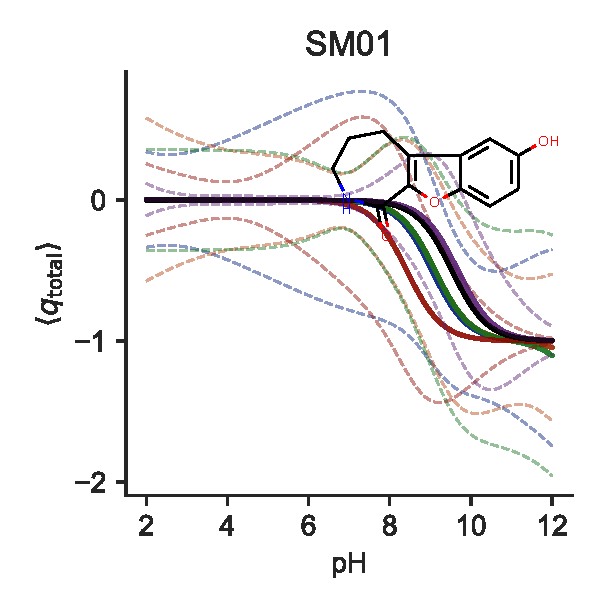
\includegraphics[width=0.33\textwidth]{Reports/overview-SM01-titration-bootstrap-molecule.pdf}
	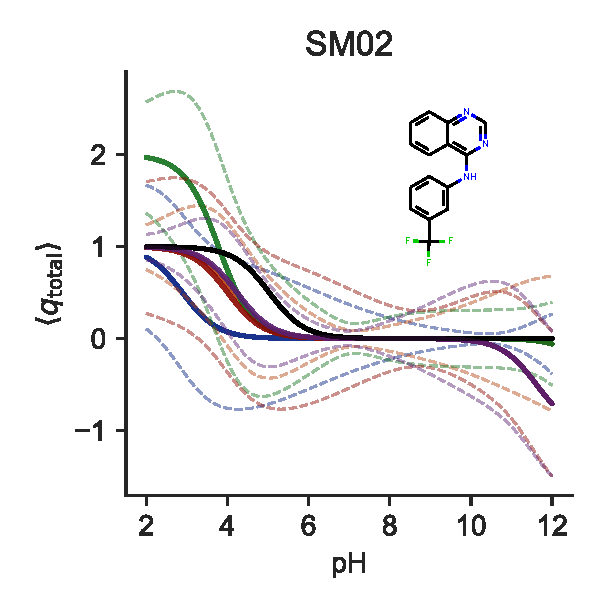
\includegraphics[width=0.33\textwidth]{Reports/overview-SM02-titration-bootstrap-molecule.pdf}
	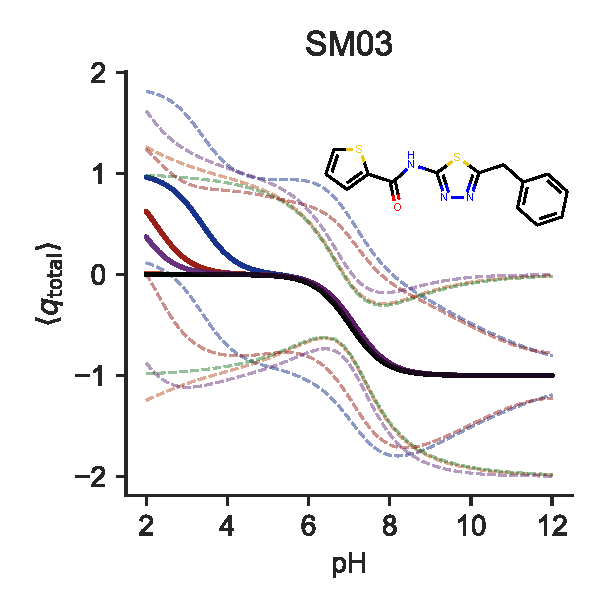
\includegraphics[width=0.33\textwidth]{Reports/overview-SM03-titration-bootstrap-molecule.pdf}	 \\
    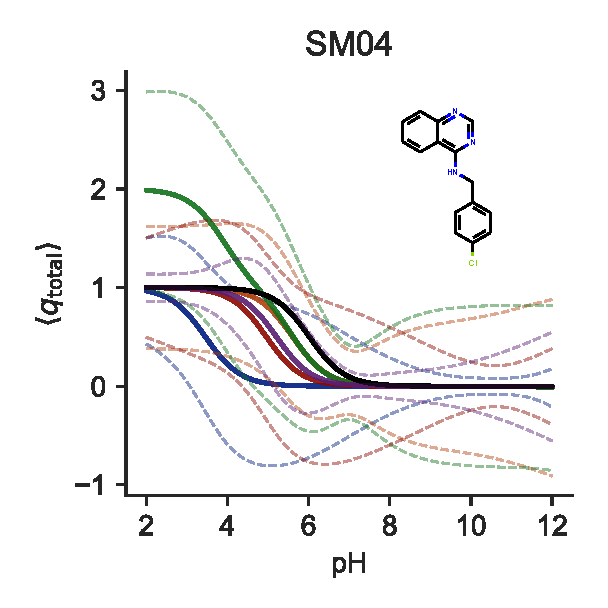
\includegraphics[width=0.33\textwidth]{Reports/overview-SM04-titration-bootstrap-molecule.pdf}
	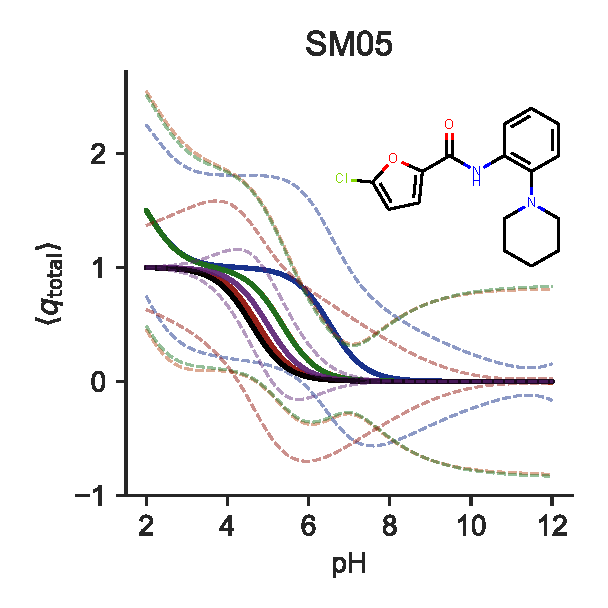
\includegraphics[width=0.33\textwidth]{Reports/overview-SM05-titration-bootstrap-molecule.pdf}
	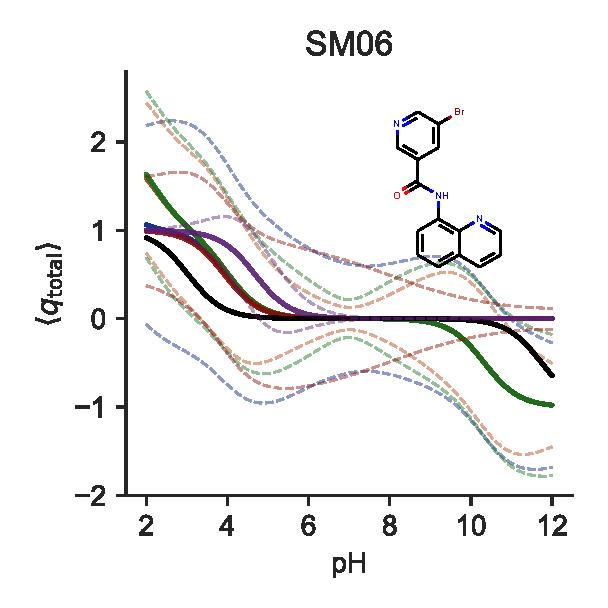
\includegraphics[width=0.33\textwidth]{Reports/overview-SM06-titration-bootstrap-molecule.pdf}	 \\
		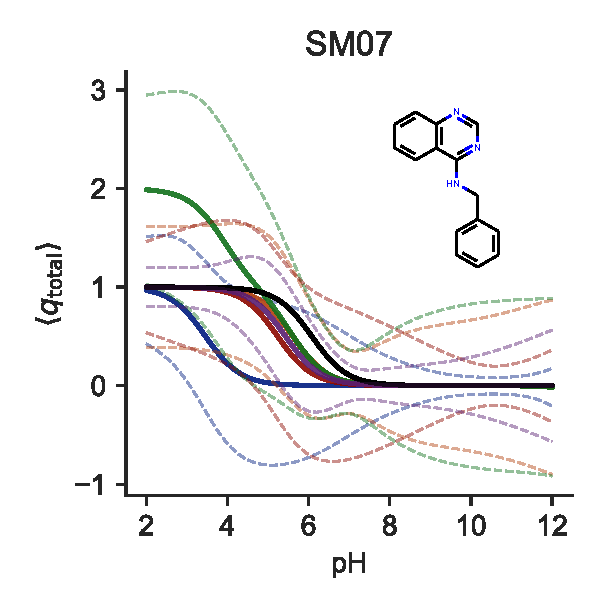
\includegraphics[width=0.33\textwidth]{Reports/overview-SM07-titration-bootstrap-molecule.pdf}
	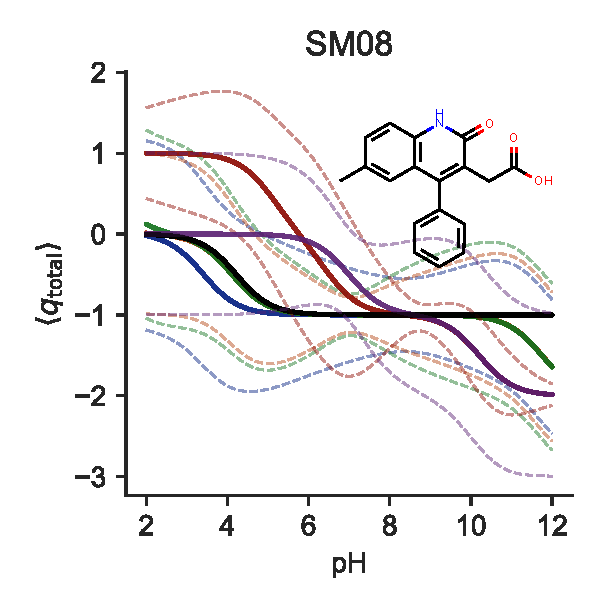
\includegraphics[width=0.33\textwidth]{Reports/overview-SM08-titration-bootstrap-molecule.pdf}
	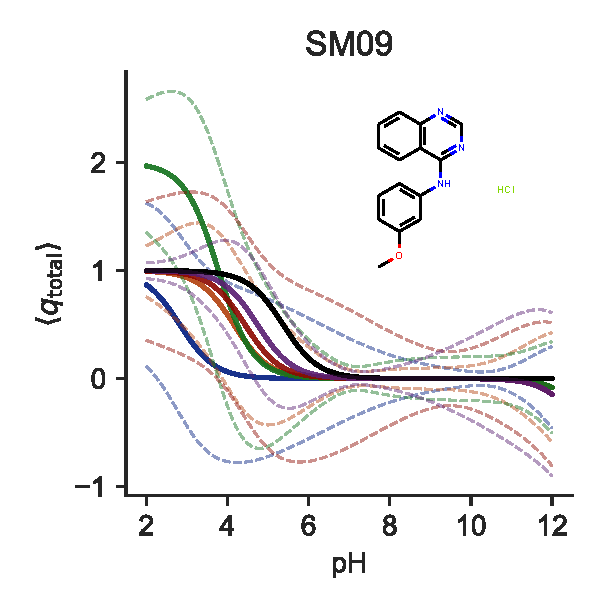
\includegraphics[width=0.33\textwidth]{Reports/overview-SM09-titration-bootstrap-molecule.pdf}	 \\
	\includegraphics[]{Reports/overview-overview-legend.pdf}
	\caption{{\bf Bootstrap titration curves for each method compared to experiment for molecules SM01-SM09.} The titration curve for each method is shown as a solid line, and 96 \% confidence intervals from bootstrap have been shown as dotted lines. Since the absolute experimental charge is not available in general, experimental curves (dashed) were aligned to each prediction independently using an integer offset that minimizes the area between curves. A numerical comparison to experiment is presented in \cref{tab:titrationcurves}.
	\label{fig:charge-curves1}}
	\end{figure}
	
	
\begin{figure}[hbt]	
	\centering
	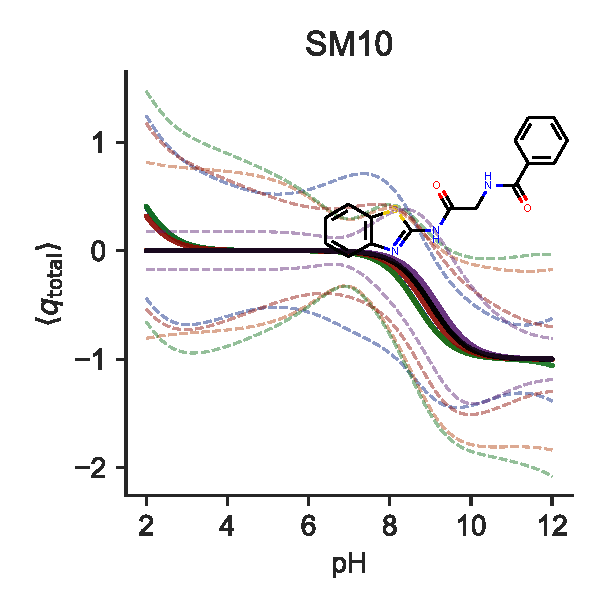
\includegraphics[width=0.33\textwidth]{Reports/overview-SM10-titration-bootstrap-molecule.pdf}
	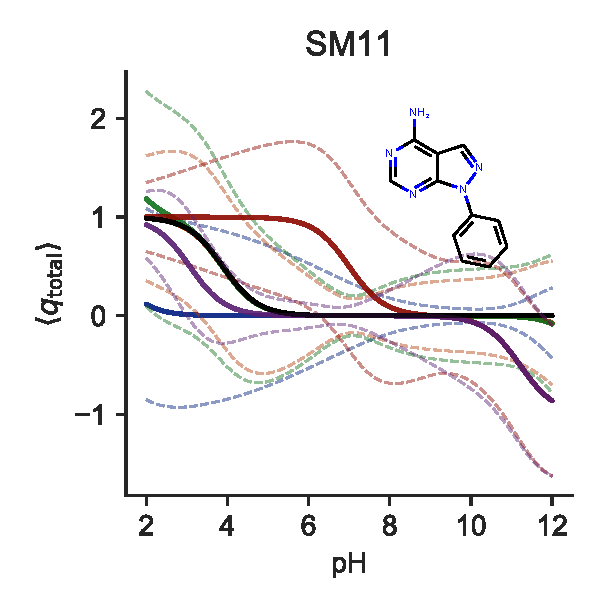
\includegraphics[width=0.33\textwidth]{Reports/overview-SM11-titration-bootstrap-molecule.pdf}
	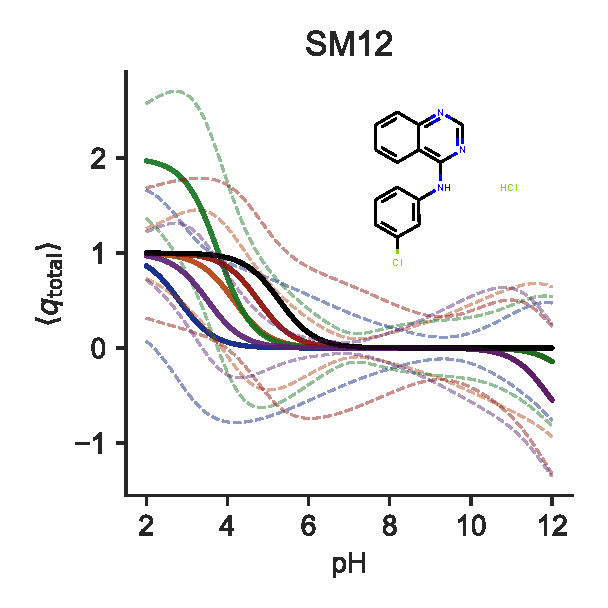
\includegraphics[width=0.33\textwidth]{Reports/overview-SM12-titration-bootstrap-molecule.pdf}	 \\
	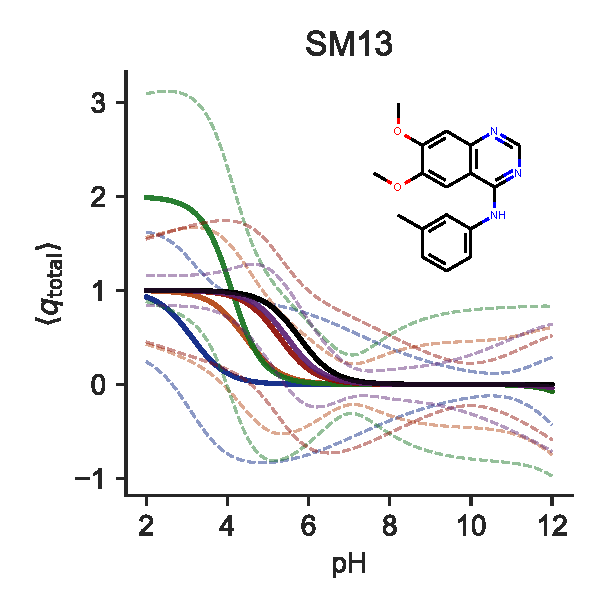
\includegraphics[width=0.33\textwidth]{Reports/overview-SM13-titration-bootstrap-molecule.pdf}
	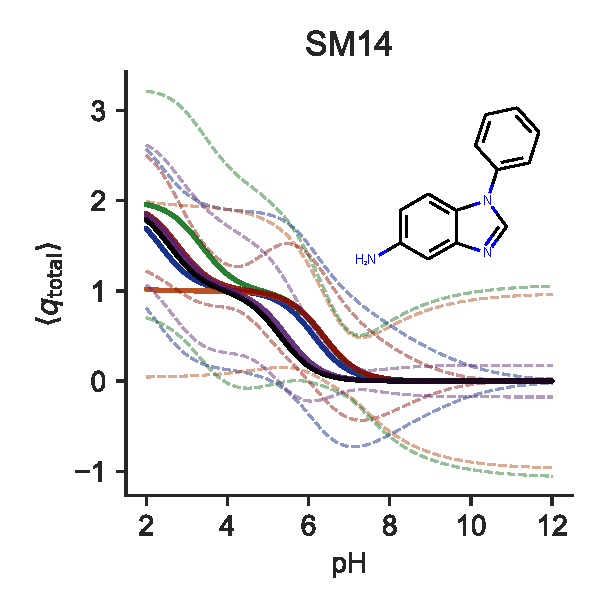
\includegraphics[width=0.33\textwidth]{Reports/overview-SM14-titration-bootstrap-molecule.pdf}
	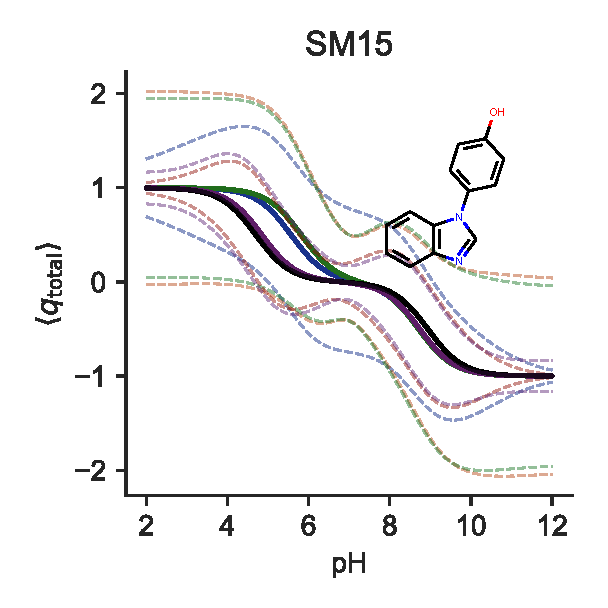
\includegraphics[width=0.33\textwidth]{Reports/overview-SM15-titration-bootstrap-molecule.pdf}	 \\
	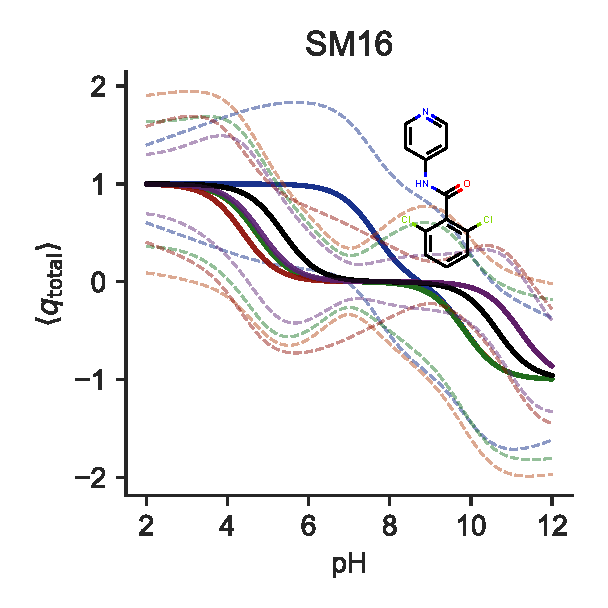
\includegraphics[width=0.33\textwidth]{Reports/overview-SM16-titration-bootstrap-molecule.pdf}
	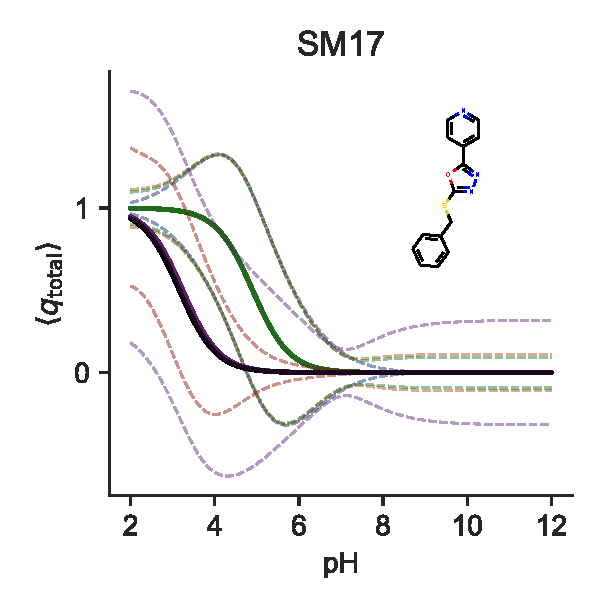
\includegraphics[width=0.33\textwidth]{Reports/overview-SM17-titration-bootstrap-molecule.pdf}
	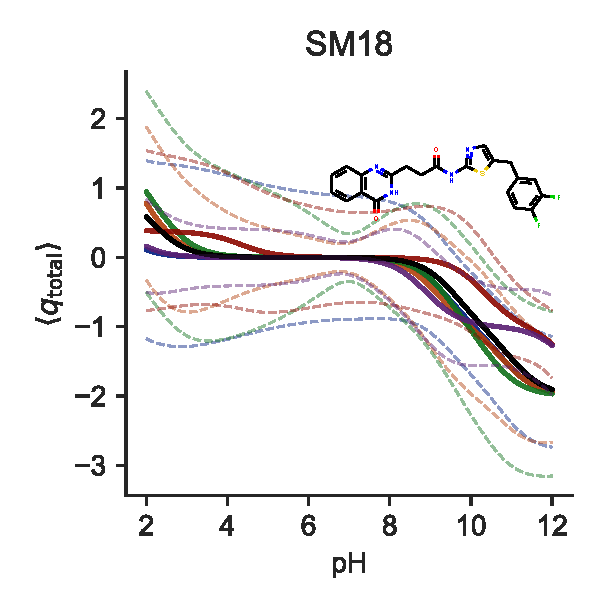
\includegraphics[width=0.33\textwidth]{Reports/overview-SM18-titration-bootstrap-molecule.pdf}	 \\
	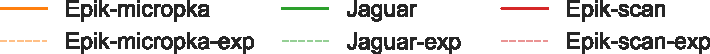
\includegraphics[]{Reports/overview-legend.pdf}

	\caption{{\bf Bootstrap titration curves for each method compared to experiment for molecules SM10-SM18.} The titration curve for each method is shown as a solid line, and 96 \% confidence intervals from bootstrap have been shown as dotted lines. Since the absolute experimental charge is not available in general, experimental curves (dashed) were aligned to each prediction independently using an integer offset that minimizes the area between curves. A numerical comparison to experiment is presented in \cref{tab:titrationcurves}.
	\label{fig:charge-curves2}}

\end{figure}
    
 \begin{figure}[hbt]	
	\centering
	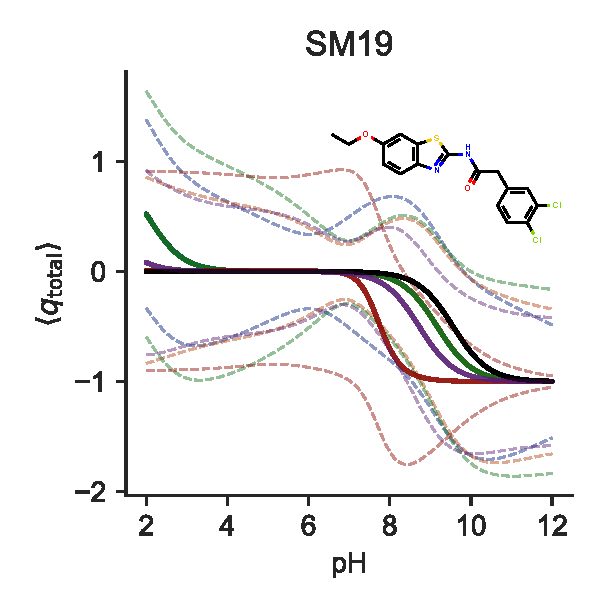
\includegraphics[width=0.33\textwidth]{Reports/overview-SM19-titration-bootstrap-molecule.pdf}
	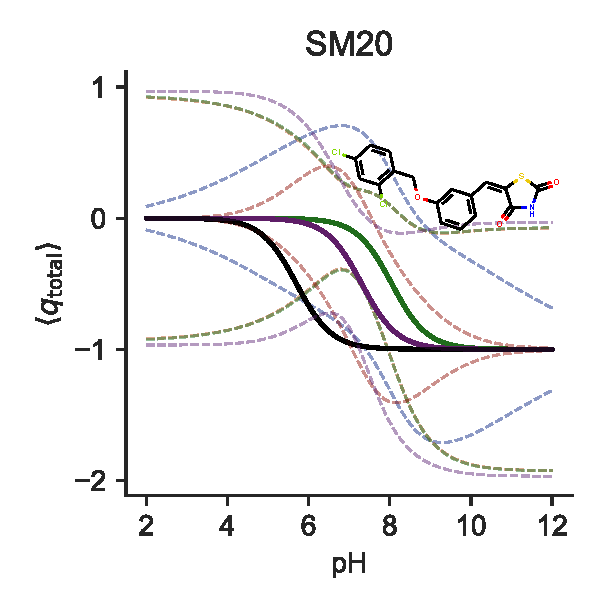
\includegraphics[width=0.33\textwidth]{Reports/overview-SM20-titration-bootstrap-molecule.pdf}
	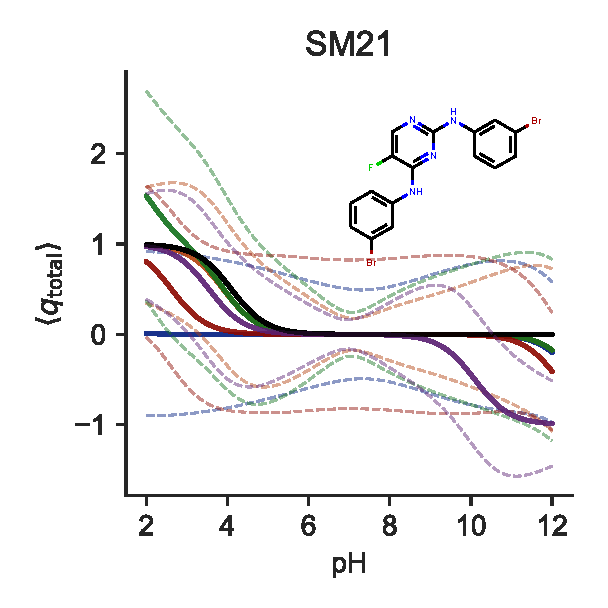
\includegraphics[width=0.33\textwidth]{Reports/overview-SM21-titration-bootstrap-molecule.pdf}	 \\
	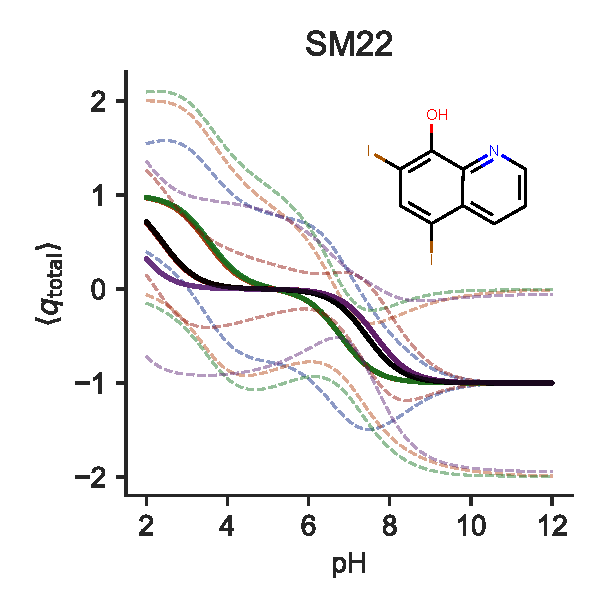
\includegraphics[width=0.33\textwidth]{Reports/overview-SM22-titration-bootstrap-molecule.pdf}
	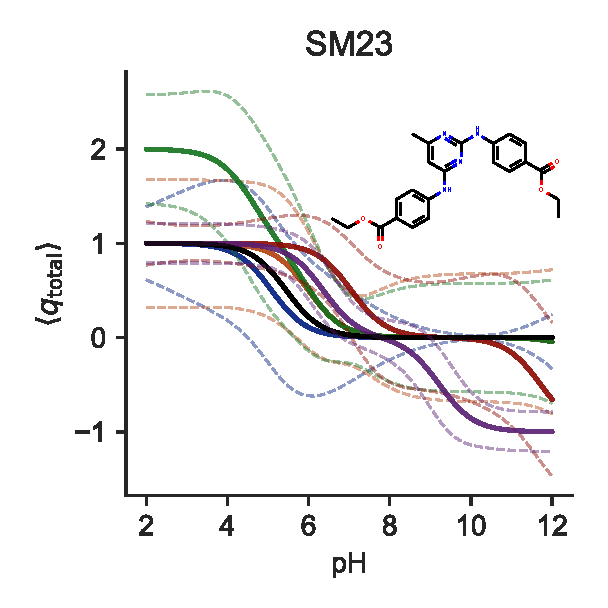
\includegraphics[width=0.33\textwidth]{Reports/overview-SM23-titration-bootstrap-molecule.pdf}
	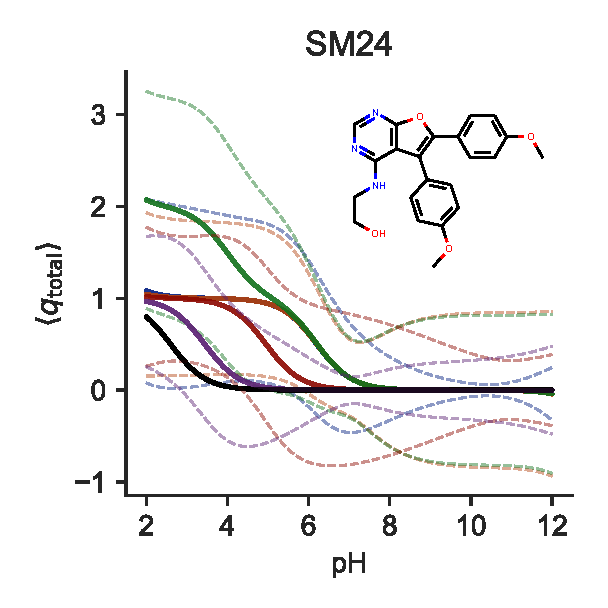
\includegraphics[width=0.33\textwidth]{Reports/overview-SM24-titration-bootstrap-molecule.pdf}	 \\
    \includegraphics[]{Reports/overview-overview-legend.pdf}

	\caption{{\bf Bootstrap titration curves for each method compared to experiment for molecules SM19-SM24.} The titration curve for each method is shown as a solid line, and 96 \% confidence intervals from bootstrap have been shown as dotted lines. Since the absolute experimental charge is not available in general, experimental curves (dashed) were aligned to each prediction independently using an integer offset that minimizes the area between curves. A numerical comparison to experiment is presented in \cref{tab:titrationcurves}.
	\label{fig:charge-curves3}}
	

\end{figure}


\section{Discussion}


\begin{itemize}
	\item How much conformation-dependence is there in Jaguar-derived pKa values (or state energies)?
	\item Does sequential scan or mean molecular charge provide better agreement with experimental macroscopic pKa values? Would it be worthwhile to develop predictive UV-metric models?
	\item Comparison of observed accuracies to previously reported/expected accuracies; expected accuracy on kinase inhibitors derived from this study
	\item How does Epik compare to Jaguar in terms of accuracy and computational cost?
	\item Discussion of outliers
\end{itemize}



\subsection{SM08 and SM11 outliers in Jaguar}

The Jaguar titration curve for molecule SM08 looks very different from the experimental curve.
%
For SM08, a pKa of 4.22 was measured experimentally.
%
If we look at the Jaguar predictions for SM08 (Figure \ref{jaguar-sm08}), this would most likely correspond to the carboxylic acid moiety of the molecule.
%
However, Jaguar predicts that the quinoline moiety in SM08 is
 titratable, and that the hydroxyl substituent is titratable as well. 
%
Experimentally, this might not be the case.
%
It seems therefore likely that Jaguar considers the titration of these
moieties too favorable compared to what is experimentally observed.

\begin{figure}[H]
    \centering
    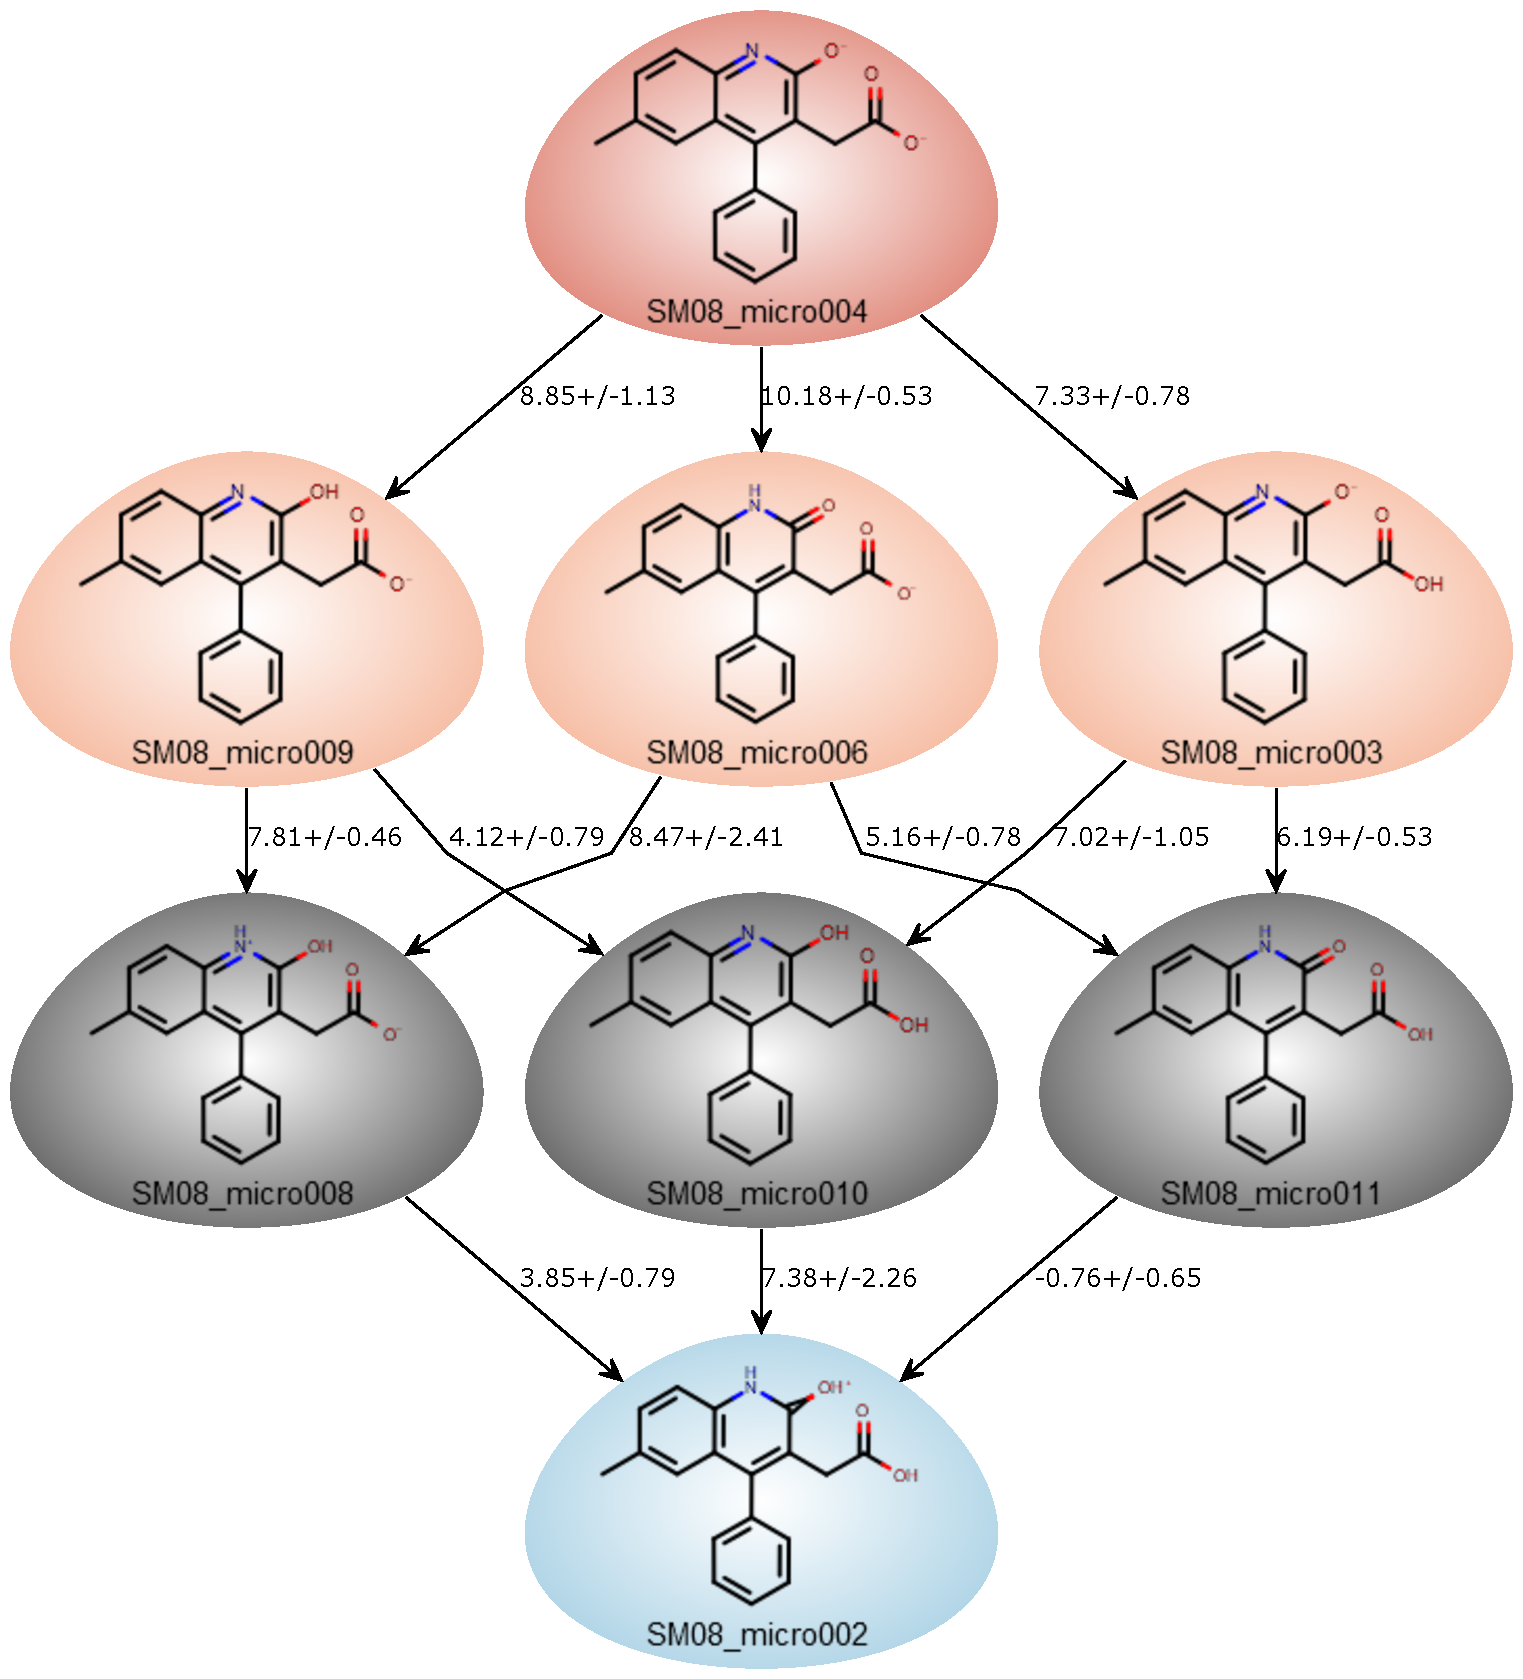
\includegraphics[scale=0.5]{Images/Graphs/SM08-Jaguar-micropka.graph.pdf}
    \caption{{\bf Jaguar titration states predicted for molecule SM08} The microscopic pKa value is shown on the \textit{right} of each arrow. The color indicates the charge (red for negative, blue for positive), where darker shades mean higher charge.}
    \label{fig:jaguar-sm08}
\end{figure}


\subsection{SM24 outliers in Epik and Epik scan}

SM24 is a molecule with a lot of potential microstates. Epik seems to perform poorly on it. Perhaps because Jaguar considered all states, it doesn't seem to do as badly as Epik.

\subsection{When Epik and Epik scan disagree}
Epik scan may sometimes produce too many pKas, oddly enough?

\subsection{Macro or micropKa, what is the realistic titration curve?}
We can generate the titration curve purely based on microscopic pKa. Alternatively,
we can use the macroscopic pKa generated using the equation \cref{eq:macropka}.

\subsection{Problematic Lewis structures}

Some low probability structures produced by Epik included questionable protonation states of a heterycyclic moiety, present in SM03 and SM18 ( \Cref{fig:lewis-structure-SM03-SM18}).  The issue leads to a pentavalent nitrogen.



\begin{figure}[H]	
\centering
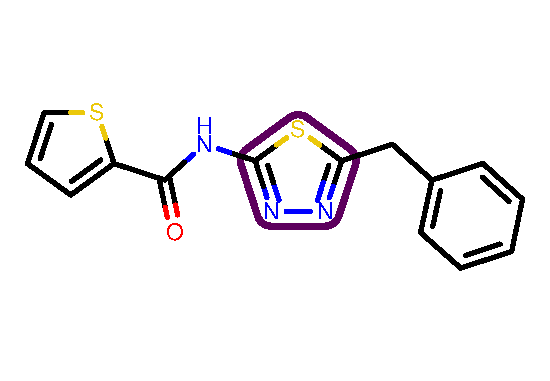
\includegraphics[width=0.33\textwidth]{Images/Molecules/SM03-smarts.pdf}
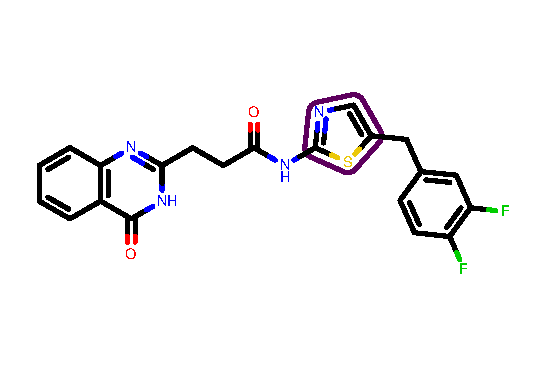
\includegraphics[width=0.33\textwidth]{Images/Molecules/SM18-smarts.pdf}
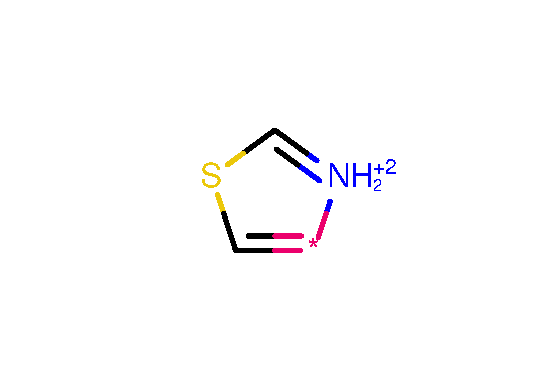
\includegraphics[width=0.33\textwidth]{Images/Molecules/lewis-problem.pdf}
\caption{{\bf Problematic lewis structure generated by Epik.}
Epik generated protonation states with invalid Lewis structure for SM03 and SM18, with a pentavalent nitrogen present in the thiazole/thiadiazole (the protonation pattern displayed on the right). One of these was also present in the set provided as part of SAMPL6  microstates, namely SM03\textunderscore{}micro021. A valid Lewis structure could not be figured out for this protonation state.}
\label{fig:lewis-structure-SM03-SM18}
\end{figure}		

\subsection{Descriptor analysis}
\begin{itemize}
	\item which moieties are harder to predict?
	\item Do certain descriptors correlate with variance/absolute errors?
	\item Do number of rotatable bonds affect epik/jaguar results (conformations missing from prediction)?
\end{itemize}


\subsection{Suggestions for future challenges}
\begin{itemize}
	\item Future challenges could benefit from NMR experiments for microstates
	\item Potentiometric titrations could capture states that may have been left out
	\item Probabilistic models (i.e. bayesian hierarchical models) could be constructed for the analysis of experiments. 
\end{itemize}

\section{Conclusions}

\begin{itemize}
	\item Epik and Jaguar perform well when matching both pKa and curves
	\item Microscopic pKa comparison directly to macroscopic may be deceiving, so the titration curve pose an alternative interpretation that can help assess
	\item Epik has a few artifacts (weird states, state penalties)
	\item future challenges could benefit from more NMR experiments and potentiometric titration data
	\item How a future challenge could make this easier
\end{itemize}


\section{Methods}

\subsection{Epik micropKa predictions}
\begin{itemize}
	\item were performed between pH 2-12
	\item Reported states with a minimum population of $e^{-10/RT}$
	\item States proposed by SAMPL6 but not predicted by Epik were not considered in analysis.
	      
\end{itemize}

\subsection{Epik scan: Sequential titration of dominant species} 


Started at pH 7.0, add protons sequentially. 
%
Produces the dominant microspecies as a way to mimic the likely macrostate.
%


\subsection{Jaguar: Ab initio quantum chemical pKa predictions}
\begin{itemize}
	\item Ran using default settings (5 conformations) for each of the pre-enumerated specified microstate pairs.
	\item Input structures were first minimized using MMFF.
	\item Additional minimization was performed for structures for which scf/geopt did not converge
\end{itemize}




%%%%%%%%%%%%%%%%%%%%%%%%%%%%%%%%%%%%%%%%%%%%%%%%%%%%%%%%%%%%%%%%%%%%%%%%%%%%%%%%%%%%%%%%%%%%%%%%%%%%%
% Code and Data Availability
%%%%%%%%%%%%%%%%%%%%%%%%%%%%%%%%%%%%%%%%%%%%%%%%%%%%%%%%%%%%%%%%%%%%%%%%%%%%%%%%%%%%%%%%%%%%%%%%%%%%%%

\section{Code and data availability}

\begin{itemize}
	\item Input files and analysis scripts are available at \href{https://github.com/choderalab/SAMPL6-reference-pka-calculations}{https://github.com/choderalab/SAMPL6-reference-pka-calculations}
	\item Our analysis methods have been packaged together in the titrato library, available at \href{https://github.com/choderalab/titrato}{https://github.com/choderalab/titrato}
\end{itemize}

%%%%%%%%%%%%%%%%%%%%%%%%%%%%%%%%%%%%%%%%%%%%%%%%%%%%%%%%%%%%%%%%%%%%%%%%%%%%%%%%%%%%%%%%%%%%%%%%%%%%%%
% Author Contributions 
%%%%%%%%%%%%%%%%%%%%%%%%%%%%%%%%%%%%%%%%%%%%%%%%%%%%%%%%%%%%%%%%%%%%%%%%%%%%%%%%%%%%%%%%%%%%%%%%%%%%%%
\section{Author Contributions}

\todo[inline]{(Follow the \href{http://www.cell.com/pb/assets/raw/shared/guidelines/CRediT-taxonomy.pdf}{CRediT Taxonomy})}

%%%%%%%%%%%%%%%%%%%%%%%%%%%%%%%%%%%%%%%%%%%%%%%%%%%%%%%%%%%%%%%%%%%%%%%%%%%%%%%%%%%%%%%%%%%%%%%%%%%%%%
% Acknowledgments 
%%%%%%%%%%%%%%%%%%%%%%%%%%%%%%%%%%%%%%%%%%%%%%%%%%%%%%%%%%%%%%%%%%%%%%%%%%%%%%%%%%%%%%%%%%%%%%%%%%%%%%
\section{Acknowledgments}

ASR, MI, AR, PBG, and JDC acknowledge support from the Sloan Kettering Institute.
JDC acknowledges support from NIH grant P30 CA008748.

%%%%%%%%%%%%%%%%%%%%%%%%%%%%%%%%%%%%%%%%%%%%%%%%%%%%%%%%%%%%%%%%%%%%%%%%%%%%%%%%%%%%%%%%%%%%%%%%%%%%%%
% Disclosures 
%%%%%%%%%%%%%%%%%%%%%%%%%%%%%%%%%%%%%%%%%%%%%%%%%%%%%%%%%%%%%%%%%%%%%%%%%%%%%%%%%%%%%%%%%%%%%%%%%%%%%%
\section{Disclosures}

JDC is a member of the Scientific Advisory Board for Schr\"{o}dinger, LLC.

\bibliography{sampl6-pKa-prediction}

%%%%%%%%%%%%%%%%%%%%%%%%%%%%%%%%%%%%%%%%%%%%%%%%%%%%%%%%%%%%
%%% APPENDICES
%%%%%%%%%%%%%%%%%%%%%%%%%%%%%%%%%%%%%%%%%%%%%%%%%%%%%%%%%%%%


\appendix

\section{Supplementary Information}



% \documentclass[11pt,final]{article}
\renewcommand{\familydefault}{\sfdefault}
\usepackage[utf8]{inputenc}
\usepackage[english]{babel}
\usepackage[showframe]{geometry}
\geometry{letterpaper}
\geometry{margin=1in}
\usepackage{graphicx}

\begin{document}
\newcommand{\molid}{SM01}
\newcommand{\methoda}{Epik-TypeI}
\newcommand{\methodb}{Jaguar-TypeI}
\newcommand{\methodc}{Epik-TypeII}
\newcommand{\methodd}{Epik-TypeIII}

\noindent 
\begin{minipage}[s]{0.35\textwidth}\centering
\includegraphics[width=\textwidth]{\molid-molecule.png}
\end{minipage}
\begin{minipage}[s]{0.35\textwidth}
\includegraphics[width=\textwidth]{overview-virtual-titration-\molid.png}
\end{minipage}
\begin{minipage}[s]{0.23\textwidth}
\includegraphics[width=\textwidth]{overview-legend-\molid.png}
\end{minipage}

\begin{minipage}[s]{\textwidth}\centering
{\textbf \methoda}
\end{minipage}

\noindent
\begin{minipage}[s]{0.32\textwidth}\centering
\includegraphics[width=\textwidth]{\methoda-virtual-titration-\molid.png}
\end{minipage}
\begin{minipage}[s]{0.32\textwidth}
\includegraphics[width=\textwidth]{\methoda-free-energy-\molid.png}
\end{minipage}
\begin{minipage}[s]{0.32\textwidth}
\includegraphics[width=\textwidth]{\methoda-populations-\molid.png}
\end{minipage}

\begin{minipage}[s]{\textwidth}\centering
{\textbf \methodb}
\end{minipage}

\noindent
\begin{minipage}[s]{0.32\textwidth}\centering
\includegraphics[width=\textwidth]{\methodb-virtual-titration-\molid.png}
\end{minipage}
\begin{minipage}[s]{0.32\textwidth}
\includegraphics[width=\textwidth]{\methodb-free-energy-\molid.png}
\end{minipage}
\begin{minipage}[s]{0.32\textwidth}
\includegraphics[width=\textwidth]{\methodb-populations-\molid.png}
\end{minipage}

\begin{minipage}[s]{\textwidth}\centering
{\textbf \methodc}
\end{minipage}

\noindent
\begin{minipage}[s]{0.32\textwidth}\centering
\includegraphics[width=\textwidth]{\methodc-virtual-titration-\molid.png}
\end{minipage}
\begin{minipage}[s]{0.32\textwidth}
\includegraphics[width=\textwidth]{\methodc-free-energy-\molid.png}
\end{minipage}
\begin{minipage}[s]{0.32\textwidth}
\includegraphics[width=\textwidth]{\methodc-populations-\molid.png}
\end{minipage}

\begin{minipage}[s]{\textwidth}\centering
{\textbf \methodd}
\end{minipage}

\noindent
\begin{minipage}[s]{0.32\textwidth}\centering
\includegraphics[width=\textwidth]{\methodd-virtual-titration-\molid.png}
\end{minipage}
\begin{minipage}[s]{0.32\textwidth}
\includegraphics[width=\textwidth]{\methodd-free-energy-\molid.png}
\end{minipage}
\begin{minipage}[s]{0.32\textwidth}
\includegraphics[width=\textwidth]{\methodd-populations-\molid.png}
\end{minipage}
\end{document}






\begin{itemize}
	\item Titration curves and free energy plots for each compound, by each method
	\item The mean charge/deviation curves for each compound and each method
	\item .mae and .sdf files with results
	\item scripts and or jupyter notebooks for analysis
	\item csv version of tables
\end{itemize}

\end{document}
